\csname documentclass\endcsname[../main.tex]{subfiles}
\graphicspath{{\subfix{../images/}}}
\begin{document}

In this section, we will present design choices, explain the architecture behind them and how they were implemented. The architecture flows through data storage and collection, data analysis, predictive modelling, and traffic simulation. We also discuss the advantages and disadvantages of certain decisions and challenges encountered.

Details of the hardware and software used for this project to ensure reproducibility are available in Appendix \ref{appdx:c}.

\textbf{A note to the reader:} Due to the research-oriented nature of this project, design and implementation were closely intertwined. Therefore, they are presented sequentially rather than in separate sections.

\subsection{Data Storage}
A dedicated database solution is essential for the project due to the large amount of data that must be collected and organised in a single, easy-to-access location. The data collected ranges from historical traffic records to event schedules, which must be stored consistently. As we are working with time-series data, a database system specialised in this type of data will be the most efficient, which, also being a NoSQL database, allows for our varied data structure. The most important requirement is a solution that efficiently handles temporal queries and supports quick querying over time windows.

\paragraph{Choice and Implementation} InfluxDB \cite{noauthor_influxdb_2022} was selected for suitability with timestamped data and easy integration with a data processing pipeline. InfluxDB was deployed on an external server to support our requirements, allowing us to access it remotely and separate the data workload from our main machine, leading to higher performance.

\subsection{Data Collection Pipeline}
Here, we describe our data collection pipeline. For the project, we require three types of data: traffic, weather, and event schedules. While focused on creating a prototype, we collected data from one city: Manchester.

\subsubsection{Traffic Data}
We require historical traffic data from Manchester. Most common sources of traffic data (Google, TomTom \cite{tomtom}) are either closed-source or only provide real-time data. However, A prior university project was completed as part of an EU-funded project to place sensors around Manchester and make these openly available, Manchester-I \cite{noauthor_manchester-i_nodate}. They provide data across traffic, weather, air quality and hydrology. For our purposes, we will only collect traffic data, for which sensors are placed across the city that provide both speed and count data split by lane direction and vehicle type, providing observations (data points) every 5 minutes, up to about 4 years of historical data.

\paragraph{Data Collected} Manchester-I has several traffic sensor deployment projects. Out of these, the Drakewell project has deployed many sensors across Manchester in partnership with \abbrev{Transport for Greater Manchester}{TfGM} \cite{noauthor_bee_nodate}. This project provides the most significant number of sensors and allows us to work with a single, more interpretable data structure. We therefore decided to collect all the data from the sensors on this project, filtering to car traffic. We present an example of the data structure in \tab{traffic_influx}.

\begin{table}[!ht]
    \centering
    \caption{Example traffic data record stored in InfluxDB.}
    \label{table:traffic_influx}
    \resizebox{0.5\textwidth}{!}{%
    \begin{tabular}{ll}
        \toprule
        \textbf{Field} & \textbf{Value} \\
        \midrule
        \_measurement & Traffic \\
        \_time & 2023-12-07T12:40:00.000Z \\
        value & 72.4 \\
        \addlinespace
        \multicolumn{2}{l}{\textbf{Tags}} \\
        \midrule
        platform\_id & drakewell\_\_1328 \\
        platform\_label & Drakewell 1328 \\
        platform\_description & Automatic Traffic Counter \\
        location & [-1.9739, 53.582] \\
        sensor\_id & avgspeed\_sw \\
        sensor\_type & vehicle-speed \\
        unit & kilometre-per-hour \\
        \bottomrule
    \end{tabular}
    }
\end{table}


\paragraph{Collection Implementation}
We provide an architecture diagram of the collection implementation in \fig{Manchester-i}. Manchester-I provides an API from which we can fetch the data. We use this API to fetch the data using a Python script, which converts it into an appropriate form for InfluxDB and writes it to the database. The structure of data in Manchester-I (Platforms -> Sensors -> Observations) requires an iterative and hierarchical approach to enable data fetching. Platforms are locations equipped with one or more sensors (for different directions or vehicle types) that capture time-series observations of speed or counts.

During development, we ran into a challenge for which two optimisations were then developed. The challenge was the time taken to perform the data collection. Since each list of observations was quite large, each of these took a long time to process. To improve this, we implemented concurrency to speed it up. The second improvement was to implement checking for existing data in our database. This allowed us to perform incremental runs of the script to finish the data collection instead of requiring it to run in one go.

\begin{figure}[!ht]
  \centering
  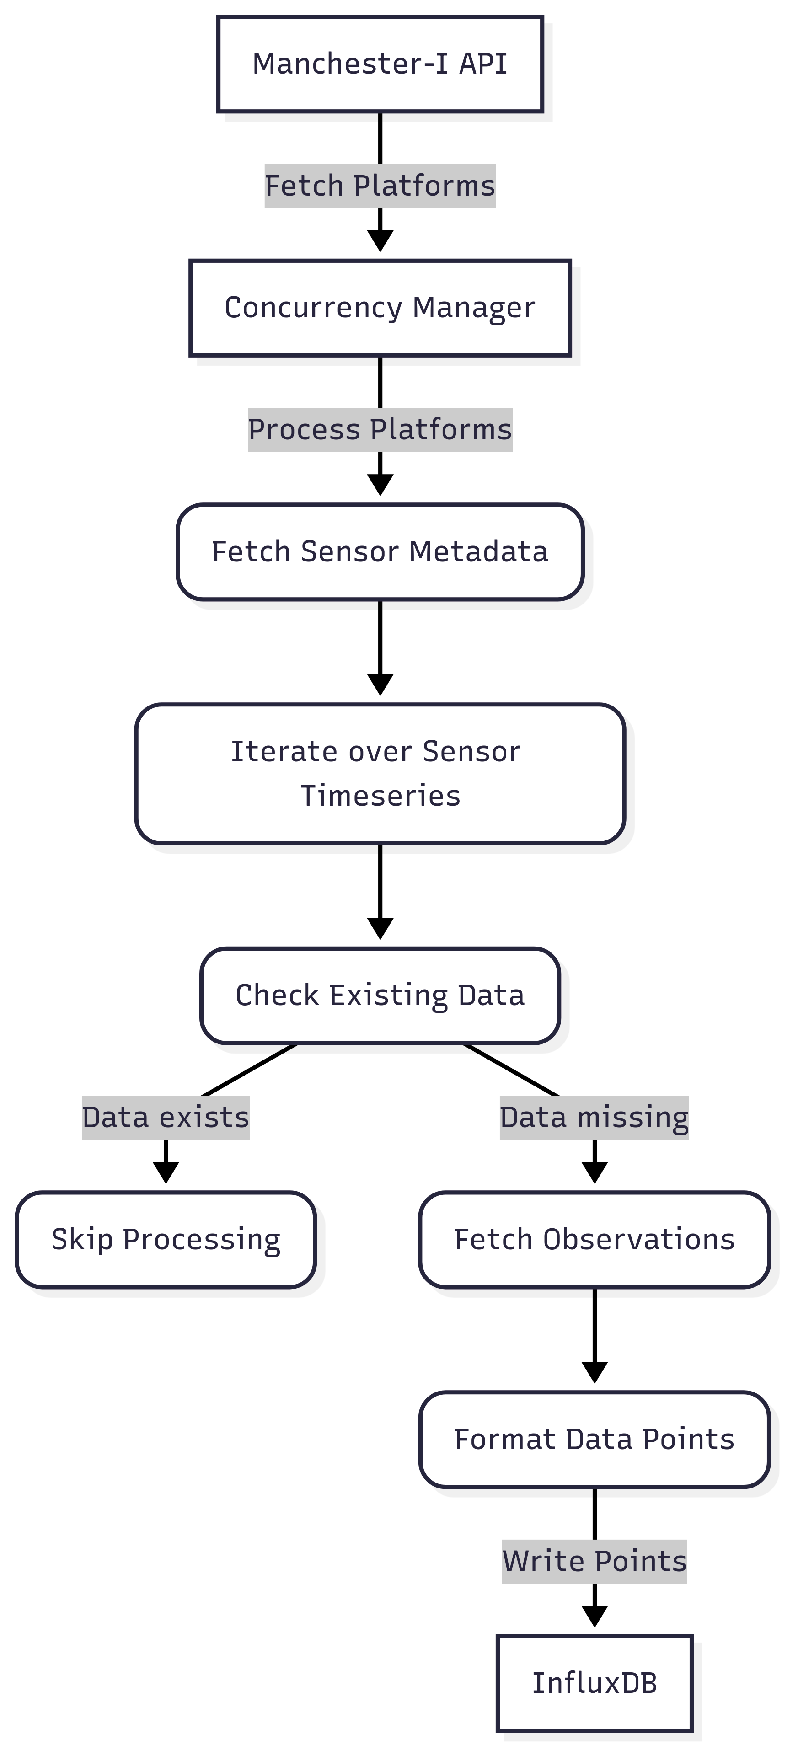
\includegraphics[width=0.4\textwidth]{images/design-implementation/manchester-i.pdf}
  \caption{Architecture diagram of Manchester-I data collection}
  \label{fig:Manchester-i}
\end{figure}

\subsubsection{Weather Data}
The literature showed the possibility of a higher prediction accuracy when including weather data. Therefore, we also collected weather data. Specifically, literature on the impact of weather on traffic specifies precipitation, wind and visibility as the most important factors \cite{bi_data-driven_2022} in traffic. For this, we decided on the Open-Meteo API, which provides free access to historical data on these fields by location (coordinates) \cite{meteo}.

\paragraph{Collection Implementation}
As this data is quite simple and uses an easy-to-access API, storing it in our database is unnecessary. Therefore, we call the API to collect the data from our DataLoader during runtime.

\subsubsection{Event Data}
Event data serves a large purpose for this project. As events are proven to have a significant impact on traffic, this data is important for our prediction models and to further test the impact of congestion management techniques. As we focus on Manchester data, we collected data from the city’s most prominent venues, which will have the most significant impact, and we can correlate venue locations with sensors. We chose two football match venues and two concert venues: Etihad Stadium, Old Trafford, Co-Op Live, and AO Arena.

\paragraph{Challenges}
Designing to collect this data is difficult for several reasons:
\begin{itemize}
    \item While some venues provide schedule data on their website, this is usually in the future and not historical data.
    \item Some APIs exist to gather historical data of events, such as API-Football \cite{football_api-football_nodate}. However, these are all paid and were not a convenient option.
    \item There was no centralised source for all these venues from which we could gather data.
    \item Some venues do not provide the start time for events on the website.
\end{itemize}

\paragraph{Data Gathering Design}
With this in mind, the design for gathering the event data required is achieved using the following two elements. We used the Wayback Machine \cite{noauthor_wayback_nodate} to access historical versions of venue websites. Regarding the actual data gathering itself, as there is no API or centralised source we can use, we use a scraping solution to extract the public data required from the HTML data of websites pertinent to each data source. For venues where start time data was unavailable, we used an approximate start time for that event category in the UK.

\paragraph{Collection Implementation}
We provide an architecture diagram of the collection implementation in \fig{event-scraping}. We scraped the required data from four sources: Concert Archives \cite{noauthor_concert_nodate}, ESPN \cite{noauthor_espn_nodate}, New York Times \cite{noauthor_NYTimes_nodate}, and Manchester United \cite{noauthor_manutd_nodate}. We collected data starting from 2020 (approximately the same period we have available traffic data) for every event at the four venues. For this task, we constructed scraping scripts for each source, using the BeautifulSoup Python library to scrape the data and then format and write it to InfluxDB. We present an example of the data structure in \tab{event_influx}. The “estimated\_attendance” field that can be seen in this data is just a placeholder at this point, and its use is explained in \textbf{\hyperref[link:llm-attendance-estimation]{LLM-Based Attendance Estimation}}.

Some sources provided the required data in a readily accessible JSON structure, while others had to be extracted from the HTML, requiring slightly different approaches. One challenge encountered during scraping was robot detection. Manually downloading pages needed to be performed where scraping failed, before being processed by our scripts.

\begin{figure}[!ht]
  \centering
  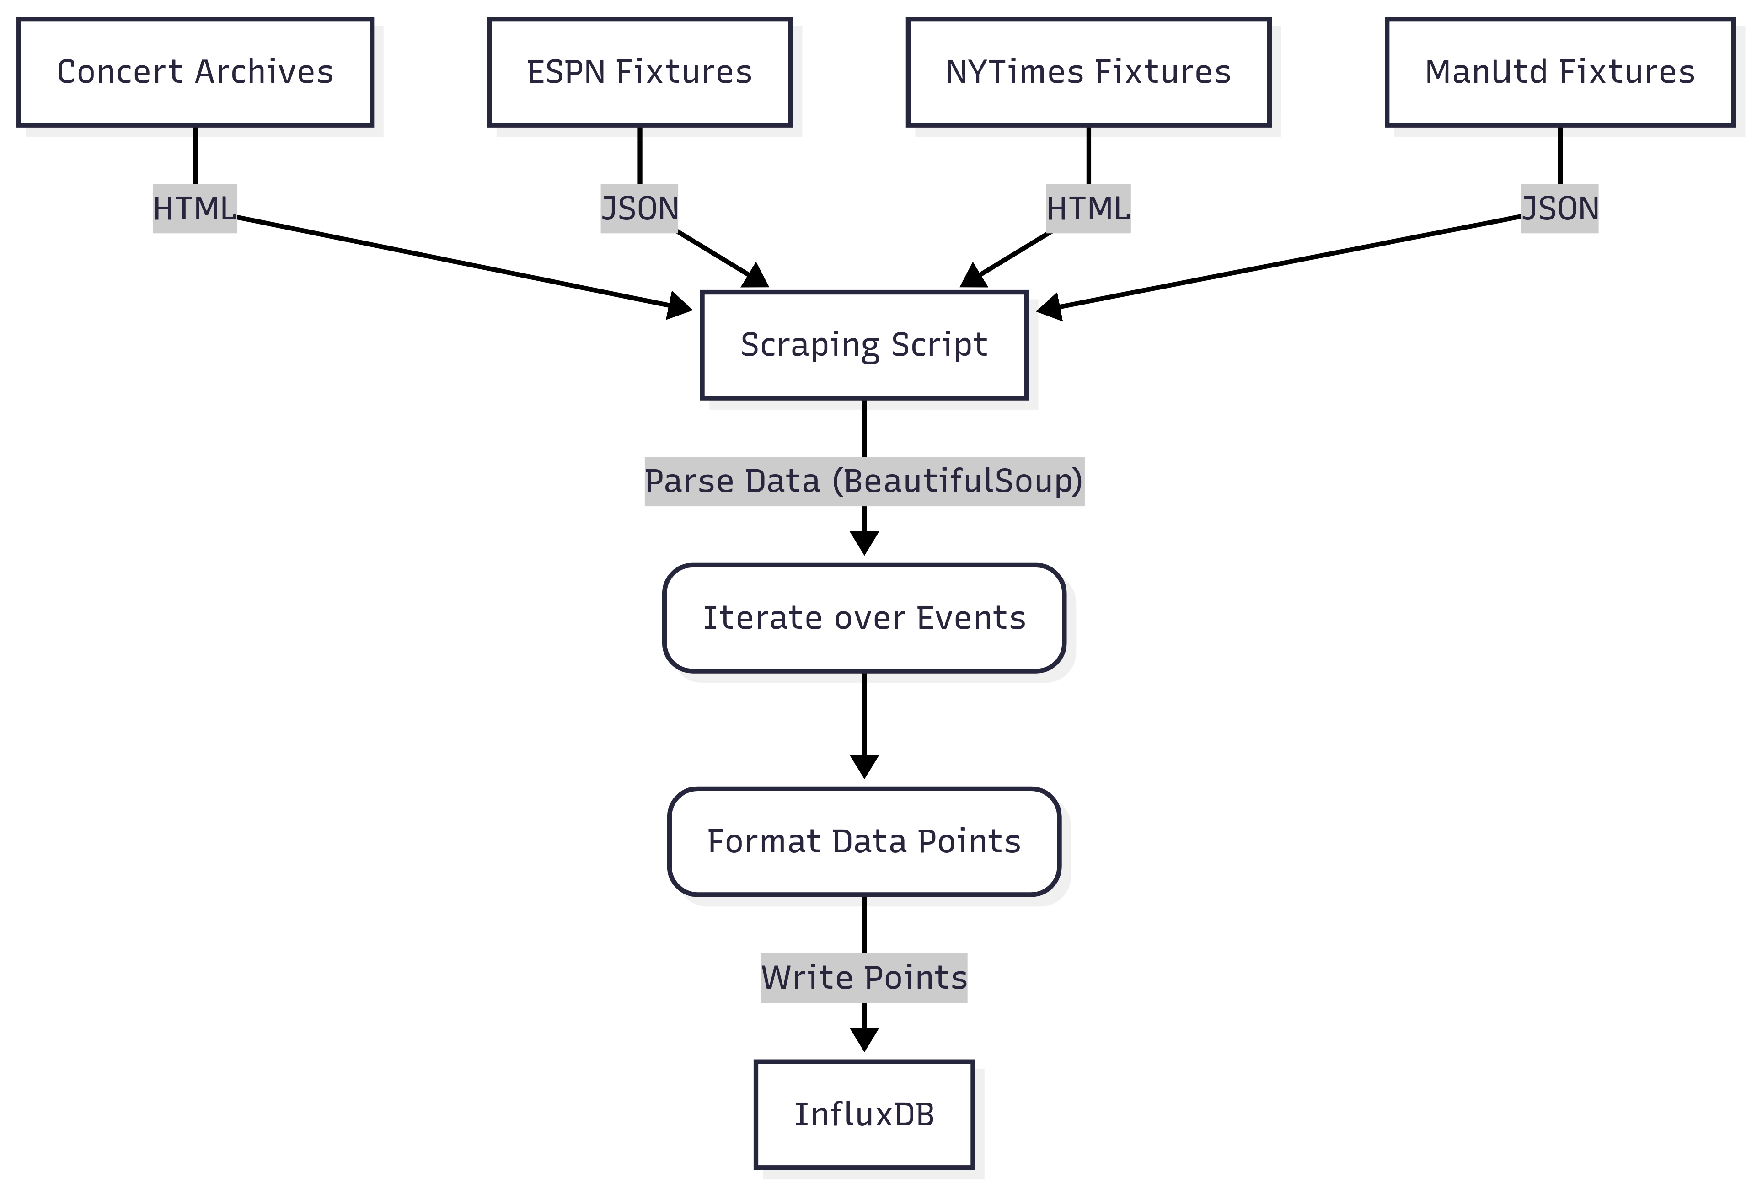
\includegraphics[width=0.8\textwidth]{images/design-implementation/event-scraping.pdf}
  \caption{Architecture diagram of event data collection}
  \label{fig:event-scraping}
\end{figure}

\begin{table}[!ht]
    \centering
    \caption{Example event data record stored in InfluxDB.}
    \label{table:event_influx}
    \resizebox{0.45\textwidth}{!}{%
    \begin{tabular}{ll}
        \toprule
        \textbf{Field} & \textbf{Value} \\
        \midrule
        \_measurement & Event \\
        \_time & 2024-05-13T04:00:00.000Z \\
        \_field & estimated\_attendance \\
        value & 0 \\
        \addlinespace
        \multicolumn{2}{l}{\textbf{Tags}} \\
        \midrule
        venue & match \\
        event\_type & OldTrafford \\
        event\_name & Arsenal @ Man Utd \\
        location & [53.463056, -2.291389] \\
        \bottomrule
    \end{tabular}
    }
\end{table}


\subsection{Data Analysis}
\label{link:data-analysis}
We will now analyse the collected data. This aims to form our research base, extract knowledge from the data, and crucially provide generalised guidance on formulating our ML models. We will focus on one venue (Etihad) and one related sensor (drakewell-1163). As our data set is extensive, we will investigate patterns from this combination, allowing us to generalise these findings to our whole data set. The Jupyter notebook with the complete analysis is available in \verb|traffic-analysis.ipynb|, located in the \verb|data_analysis| directory of the repository (\hyperref[appdx:a]{Appendix A}).

\subsubsection{Sensor and Venue Locations} We collected data from 48 platforms, each of which provides counts and speeds for each lane direction. A plot of all these locations and the locations of our chosen venues is available in \fig{map-out}, with a zoomed-in version containing venue labels in \fig{map-in}.

\begin{figure}[!ht]
  \centering
  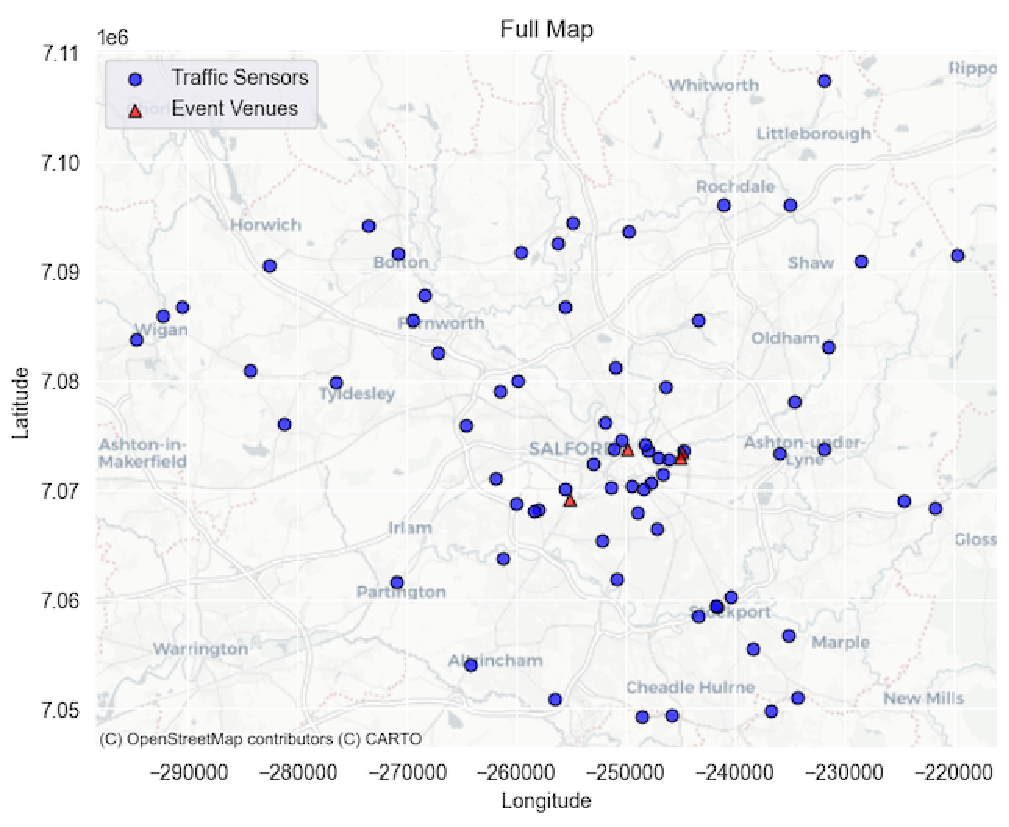
\includegraphics[width=0.7\textwidth]{images/design-implementation/map-out.pdf}
  \caption{Zoomed-out plot of traffic platforms and venues collected}
  \label{fig:map-out}
\end{figure}

\begin{figure}[!ht]
  \centering
  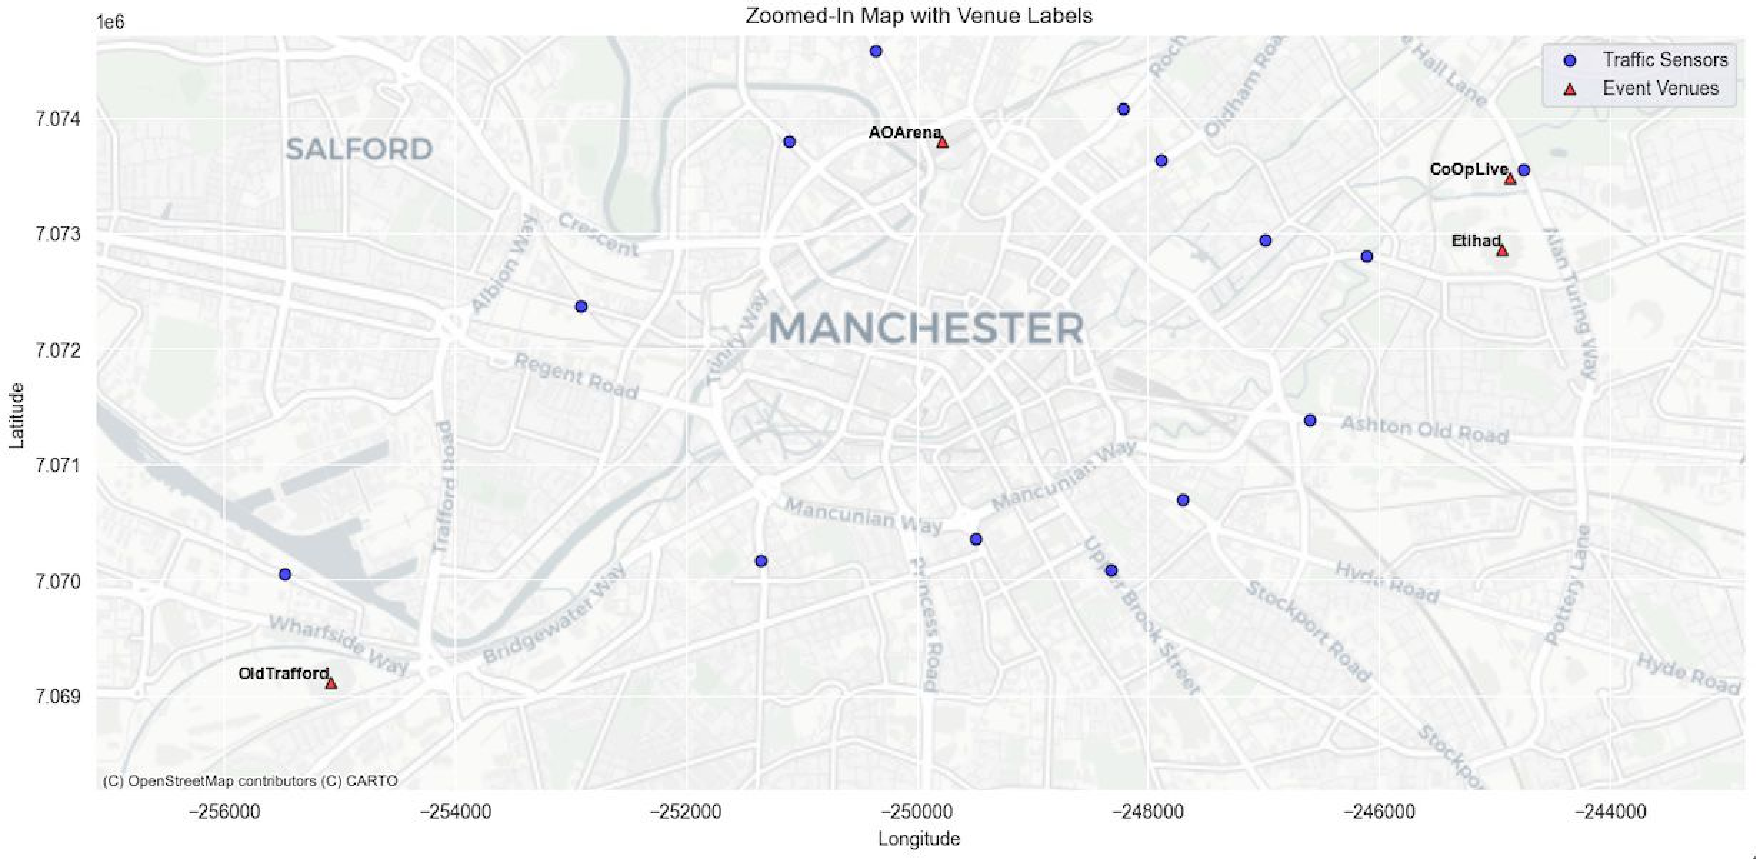
\includegraphics[width=1\textwidth]{images/design-implementation/map-in.pdf}
  \caption{Zoomed-in plot of traffic platforms and venues collected}
  \label{fig:map-in}
\end{figure}

\subsubsection{General Analysis and Preprocessing}
\label{link:data-preprocessing}
Upon exploring the traffic data, several observations can be made. The data appears consistent with expected patterns. However, notable gaps have been identified, primarily involving large recent missing data segments, despite earlier periods showing continuous data. An example is shown in \fig{traffic-speed-year}. Traffic speed data is precise, consisting only of average speeds recorded separately for each direction, while traffic counts are subdivided by vehicle type. Given this project’s scope, the analysis will be restricted to car counts and average speeds.

During preprocessing, two primary issues were observed: zero values in speed data, likely indicating sensor errors, and prolonged intervals of missing data, potentially caused by more significant sensor malfunctions. Therefore, large missing segments will be excluded entirely from the analysis, as interpolation could result in inaccuracies, and zero-valued speed entries will be removed. Count data will not require this treatment, as zero values represent valid observations and do not show sudden drops. An example is shown in \fig{traffic-count-day}.

\begin{figure}[!ht]
  \centering
  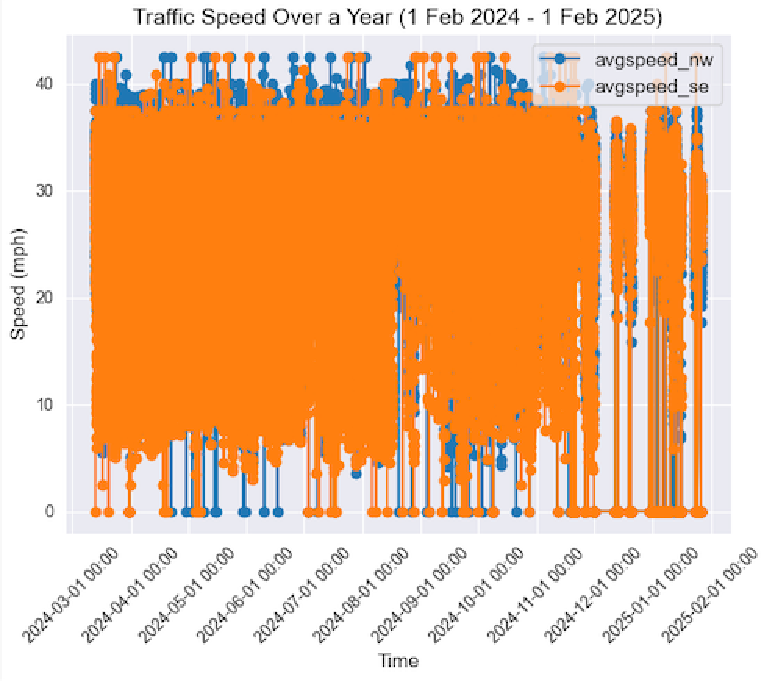
\includegraphics[width=0.7\textwidth]{images/design-implementation/traffic-speed-year.pdf}
  \caption{Plot of traffic count over a year}
  \label{fig:traffic-speed-year}
\end{figure}

\begin{figure}[!ht]
  \centering
  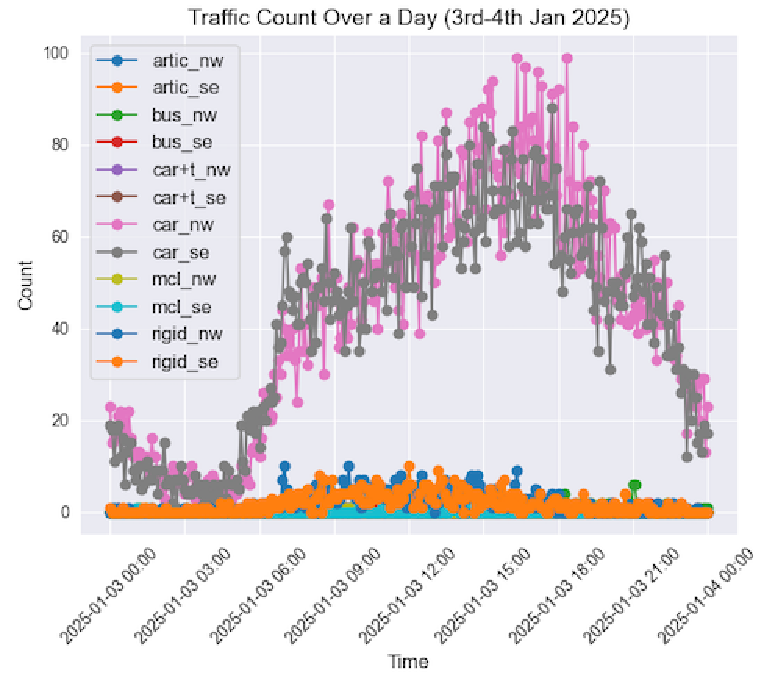
\includegraphics[width=0.7\textwidth]{images/design-implementation/traffic-count-day.pdf}
  \caption{Plot of traffic speed over a day}
  \label{fig:traffic-count-day}
\end{figure}

\subsubsection{Correlation with Events}
Next, we investigate the correlation of events with traffic data. For this, we compiled plots of the traffic data around each event in the collected data. An example of this Plot is available in \fig{traffic-event-corr}, where the red dashed line represents the event's start time. Here, we can identify that speeds tend to decrease gradually before the event time and increase afterwards before decreasing again after a few hours (presumably when the event ends). This pattern confirms that congestion occurs around events, supporting the model’s relevance. The count metric shows similar but inverse trends, but less descriptive and pronounced, which are less useful for our purpose.

\begin{figure}[!ht]
  \centering
  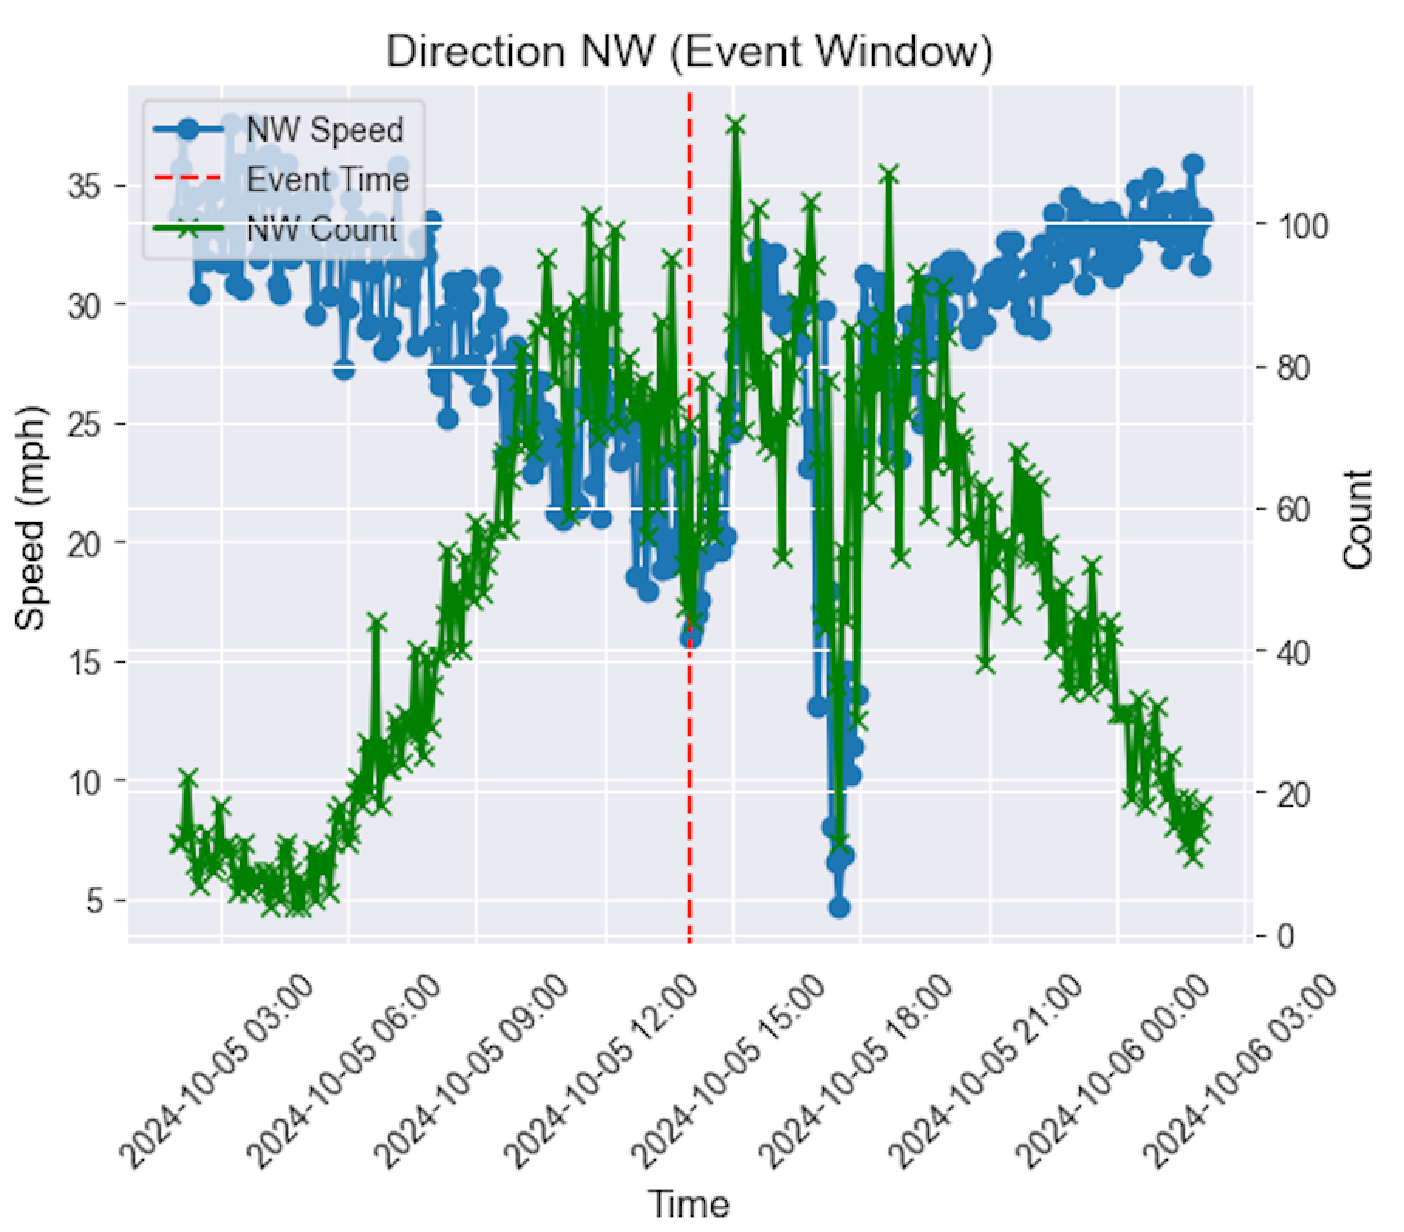
\includegraphics[width=0.6\textwidth]{images/design-implementation/traffic-event-corr.pdf}
  \caption{Plot of traffic data around an event at Etihad}
  \label{fig:traffic-event-corr}
\end{figure}

\subsubsection{Traffic Speed vs. Count Analysis}
Given the analysis in prior sections, we complete a final analysis on speed vs. count for traffic. This results from a correlation analysis that resulted in \fig{correlation} and an average correlation coefficient of -0.43. This shows that while a negative correlation is found, it is not very strong. This is expected and can be caused by external factors such as weather conditions, roadworks, or accidents, which can affect traffic speed without significantly impacting traffic count. Due to the nature of this project, reasons given earlier when performing this analysis directly in comparison with events, and given these observations, we will use traffic speed as the primary metric in our models, as this is more descriptive and has a clearer relationship with our project goal.

\begin{figure}[!ht]
  \centering
  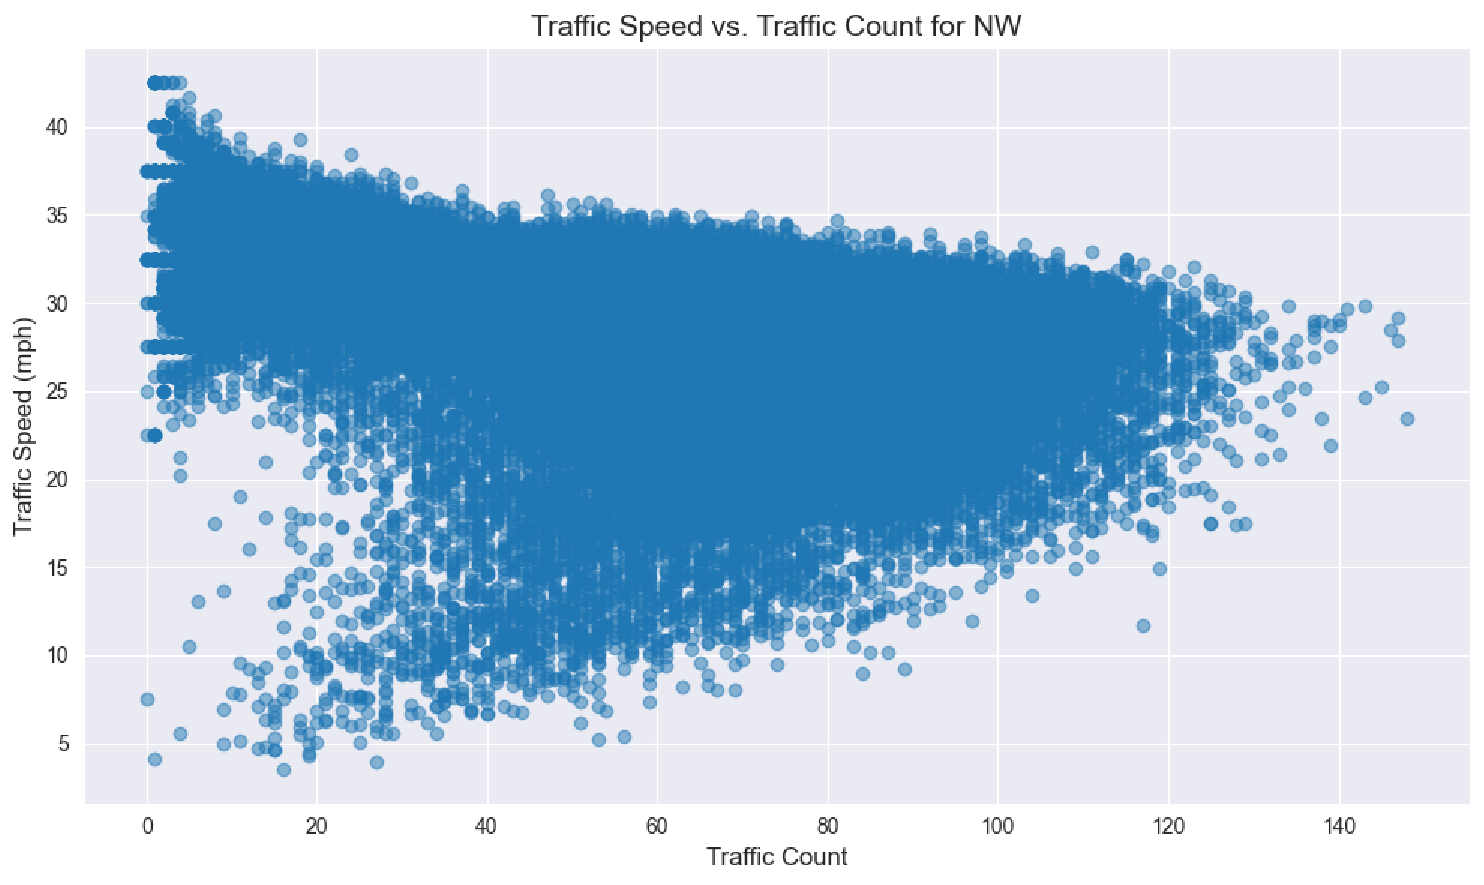
\includegraphics[width=0.8\textwidth]{images/design-implementation/correlation.pdf}
  \caption{Plot of correlation between traffic speed and traffic count for one direction}
  \label{fig:correlation}
\end{figure}


\subsection{Feature Engineering}
In this section, we will explore the feature engineering work performed for the project. Feature engineering transforms raw data into formats suitable for machine learning models \cite{noauthor_feature_2024}.

\subsubsection{Traffic Features}
Traffic features are relatively simple. We can use only the data's time as its feature. To achieve higher performance, we designed two different encodings.

\paragraph{Basic Time Encoding}
In the typical time encoding, we split the timestamp into several valuable features that the model can use to identify trends such as seasonality, differences in time of day, and weekdays vs. weekends. The complete list of features derived from the timestamp we use is as follows: year, month, day, weekday, hour, and minute.

\paragraph{Cyclic Time Encoding}
In cyclic time encoding, we use the same features but encoded in a cyclic manner (using sin and cos values) to model the cyclic trends in this data based on existing research \cite{pelletier_cyclical_2024}. We do this for the month, weekday, hour, and minute features, which allows the model to understand continuance in, for example, minutes 59 to 0. The year and day features will remain non-cyclic, as years are continuous and days are irregular depending on the month.

\subsubsection{Weather Features}
As the weather features are simple and direct, we pass the values straight through: precipitation, wind speed, and relative humidity (which identify conditions for fog).

\subsubsection{Event Features}
Event Features are the most complex due to our focus on event impact for this project. We explore two different encodings of event schedules as inputs to our models. One is a simple binary event encoding, while in the second section, we will design a custom encoding.

\paragraph{Binary Event Encoding}
In this encoding type, we utilise a single feature to represent an event affecting a time point. We use two variables to control this:
\begin{itemize}
    \item The time difference of the event to a time point: x
    \item The location distance between the event venue and a traffic sensor: y
\end{itemize}
If an event occurs within x time of a particular timepoint and the distance to it is smaller than y, then we encode this feature as True; otherwise, it is False.

\paragraph{Custom Event Encoding}
Here, we design a more complex encoding to incorporate more information into the models that could lead to higher prediction accuracies. The general idea is to provide the actual information of the time difference and location distance, the type of event, and the same binary encoding as above. This leads to four features:
\begin{itemize}
    \item The location distance to the event
    \item The time difference to the event
    \item The event type (for our data, “match” or “concert”)
    \item The binary representation, as in the earlier section
\end{itemize}
In this encoding type, a particular design decision occurs regarding which event to select when multiple events occur on the same day. As we are dealing with traffic data, we assume that the event happening closest to the venue will be the one with the most impact, and therefore, we compute the remaining features for this event. With this type of encoding, we keep the notion of a maximum time difference and distance, over which we ignore that event.

\paragraph{Implementation}
The implementation of the feature encodings for events is as follows. For every point of traffic data being used, we iterate over every event in that same timeframe, followed by:
\begin{enumerate}
    \item Computing the time difference between the event and the traffic data point
    \item Confirming if the time difference is within our maximum. If not, discard.
    \item Computing the distance difference between the event and traffic data point using the GeoPy package.
    \item Confirming if the distance difference is within our maximum. If not, discard.
\end{enumerate}

The hyperparameters of time and distance, x and y, were determined through experimentation. The maximum distance was set to 3 km, as we found no difference in accuracy from this point onwards. The maximum time was set to 12 hours, as we found events to have an effect up to then, after testing 4, 6, and 10 hours.

Once this is computed for all events, we find the event with the minimum distance and allocate the features accordingly. There are two essential aspects to note in the implementation. Firstly, the use of the time difference is not absolute; therefore, we provide the model with both the magnitude and direction of the time difference, allowing it to understand the differences between traffic before and after the event (such as traffic peaks at the event's end). Secondly, as features cannot be set to null when an event does not impact a traffic data point, we set these to a high default number to allow the model to understand that there is no impact. This is used for both the distance and time features.

\paragraph{Optimisations}
Since the feature engineering of events is highly computationally intensive (O(n\sus{2}) runtime), we implement two significant optimisations to ensure this process runs in an acceptable time.

\begin{enumerate}
    \item We use NumPy vectors to represent the data and intermediate arrays, precomputing the initial arrays whenever possible.
    \item We implement concurrency in this step to allow the feature engineering to run on multiple cores in parallel.
\end{enumerate}

\subsubsection{LLM-based Attendance Estimation}
\label{link:llm-attendance-estimation}
This section proposes a novel \abbrev{Large Language Model}{LLM}-based attendance estimation pipeline to enhance the event features. A problem faced when using event-based features is not having any information on the actual attendance of an event. While each venue has a specific capacity, events may not continuously operate at them. Given that the traffic impact is generally directly correlated with the number of attendees at an event, knowing this number could improve predictive accuracy.

\paragraph{Pipeline Design}
An architecture diagram of the proposed system is available in \fig{llm-estimation}. The pipeline gathers the event data collected and uses this to generate a prompt that will query an LLM, along with context on the task, to generate estimates of each event's attendance. The LLM is given the event name, type, venue, and date. The prompt used for this is given in \textbf{\hyperref[appdx:b]{Appendix B}}. The LLM returns the estimates in JSON format, which are extracted and then used to update the event data points in InfluxDB to contain this estimate.

\paragraph{Implementation}
This pipeline is implemented through a Python script that iterates through every event in the database and uses the above process to update them with the estimate. To interact with LLMs, we used OpenRouter, a unified API that allows access to many models with no or low cost \cite{noauthor_openrouter_nodate}. For the model, we used Gemini 2.0 Flash Lite Preview \cite{noauthor_gemini_nodate}, which was available at no cost, runs in an acceptable time (compared to a reasoning model), and returns estimates that, when manually reviewed, seem very reasonable for the venues and events in question.

\begin{figure}[!ht]
  \centering
  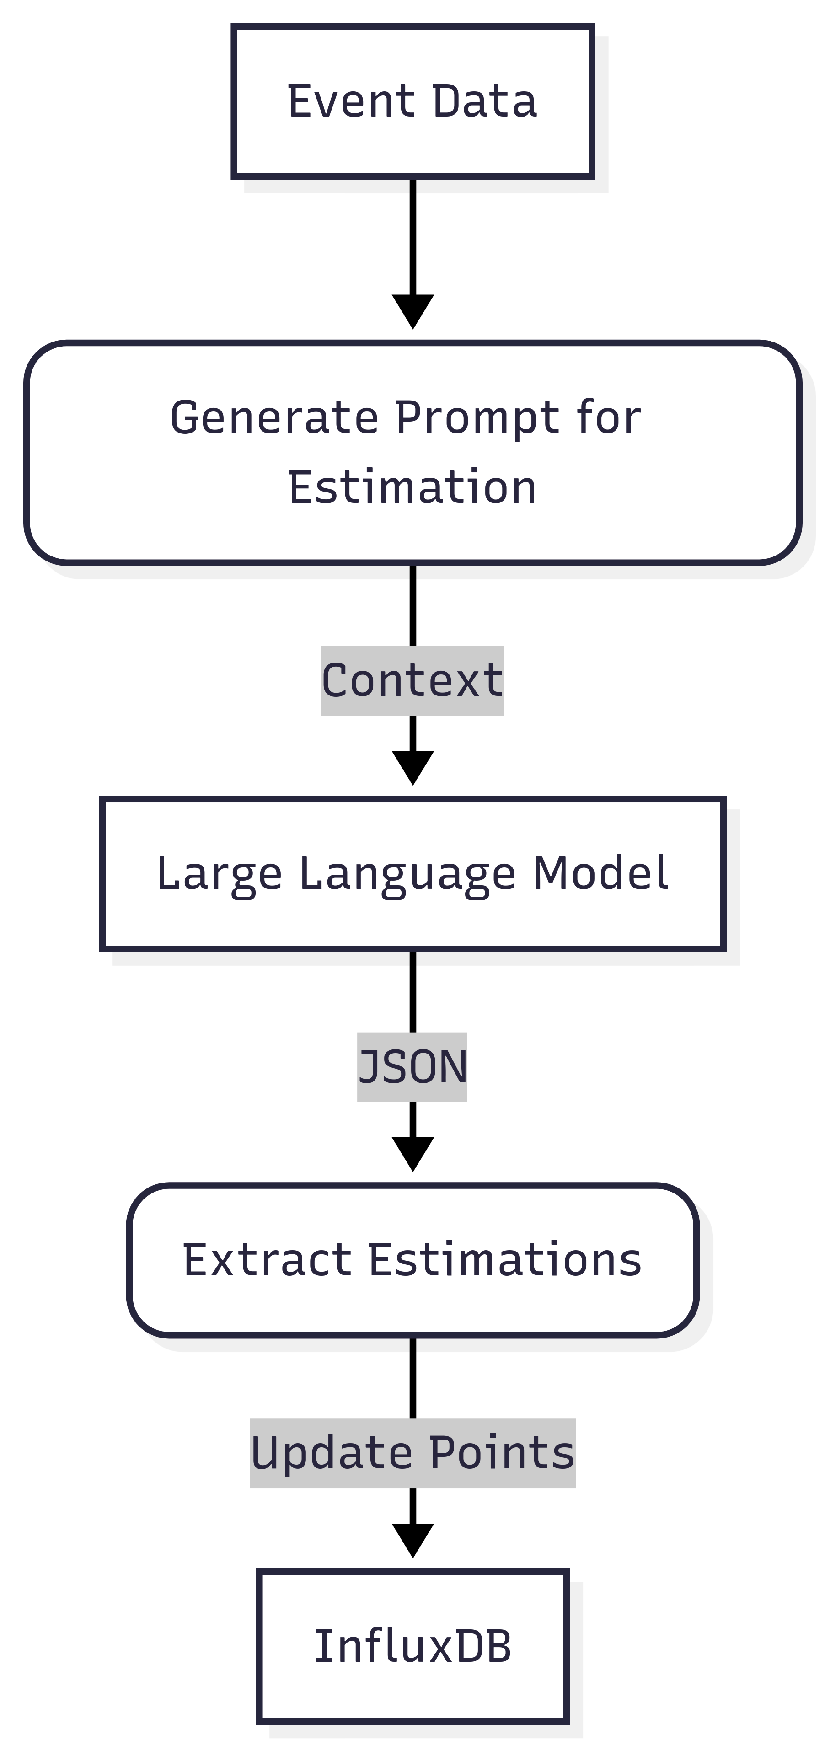
\includegraphics[width=0.3\textwidth]{images/design-implementation/llm-estimation.pdf}
  \caption{Architecture diagram of LLM-based Attendance Estimation}
  \label{fig:llm-estimation}
\end{figure}

\subsection{Predictive Modeling}
We now explain the modular approach towards the design of the predictive modelling system. This system is designed using Python. Each component has a clear responsibility: \verb|batch_training.py| handles training across multiple sensors, while \verb|train_model_nn.py| focuses on neural network training for a single sensor. \verb|predict.py| generates predictions from trained models, and \verb|model_training.py| defines the model architectures and training routines. Data ingestion is managed by \verb|data_loader.py|, and \verb|feature_engineering.py| encapsulates all transformations for traffic, event, and weather features. Additionally, \verb|create-estimations.py| estimates event attendance using LLMs (as described in the earlier sections), and \verb|config.py| forms part of a tool that centralises configuration and key management. This modular structure enables the clean separation of concerns, easier experimentation, and flexible scaling across different modelling scenarios.

\subsubsection{Design Decisions}
\paragraph{Flow Identification}
First, we discuss the identification of flow. As the data collected provides us with the traffic speed for a specific sensor in both lane directions, we must choose between combining the flow and predicting the flow irrespective of direction or treating these as two separate flows. Given the data analysis performed, where we can see different trends depending on the direction (for example, traffic incoming to a venue vs outgoing), we will treat these separately to provide greater accuracy.

\paragraph{Model Design}
Additionally, there are two options regarding model design. Firstly, a model that performs predictions across all the sensors as one big predictive model that collects all the information and then predicts based on the features in conjunction with the location of the requested sensor. Secondly, training separate models for each sensor and direction would allow for many smaller models to predict traffic at that particular sensor and direction.

While having one large model would allow for generalisation based on location, allowing nearby sensors to share traffic patterns and recognise the effects of each other, we decided to perform the training of separate models due to the following reasons:
\begin{enumerate}
    \item The data we have available for traffic is limited in locations. Most of the sensors are spread around the city, meaning the advantage stated above would not hold.
    \item Using smaller models for each sensor allows focusing specifically on patterns at each location while maintaining a much smaller, more efficient model.
\end{enumerate}

\paragraph{Model Choices}
\label{link:model-choices}
In our exploration of models for traffic speed prediction, we evaluated a wide range of neural network architectures based on our background research. These included MLPs, RNNs, LSTMs, CNNs, GNNs, and transformer-based models. These models were considered to be suitable for capturing temporal or spatial dependencies, the nature of our data, and computational requirements. We noted that while RNNs and their variants, like LSTMs, are excellent at handling sequential data, they struggle with long-term dependencies. This results in them only being able to handle short-term forecasting. CNNs and GNNs, on the other hand, require lots of data or interconnected locations to work correctly. Due to the nature of our data, these were ruled out. Transformer-based models, although state-of-the-art and very powerful, were ruled out due to their high computational cost, which may be impractical for an ITS with limited processing resources.

Given these considerations, we selected three models to implement. The first is ARIMA, the classical time-series forecasting model typically used as a benchmark. For neural networks, we settled on LSTM and MLP architectures. LSTM was chosen for its ability to capture trends in data better; however, it can only forecast short-term. MLP was selected for its efficiency in processing features (a significant focus of this project) and long-term forecasting. This selection allows us to balance computational efficiency with predictive accuracy, given data availability. Regarding short-term vs long-term forecasting, we choose to implement these two models with different types of forecasting in order to test them before deciding which to use for our congestion management design.

\subsubsection{Traditional Statistical Model (ARIMA)}
An architecture diagram for this model is provided in \fig{arima-arch}. This architecture is quite simple, as is the model itself—our dataloader queries for all the traffic data available for that sensor and direction. Once done, we preprocess according to the \textbf{\hyperref[link:data-preprocessing]{data preprocessing}}. This data is then split using a train-test split of 80-20\%, and the model is fitted on this data using an ARIMA(1,1,1) architecture. Once complete, we forecast the testing data and compare it with the actual values.

As this model works only on temporal data, we provide only the raw traffic speed values and no other features. The ARIMA(1,1,1) model was chosen as it works well with little knowledge of the underlying data trends or structure and covers all the base ARIMA features. This model was quickly abandoned, as discussed in the \textbf{\hyperref[link:arima-results]{results}}, and therefore, no optimisations past this baseline were performed.

\begin{figure}[!ht]
  \centering
  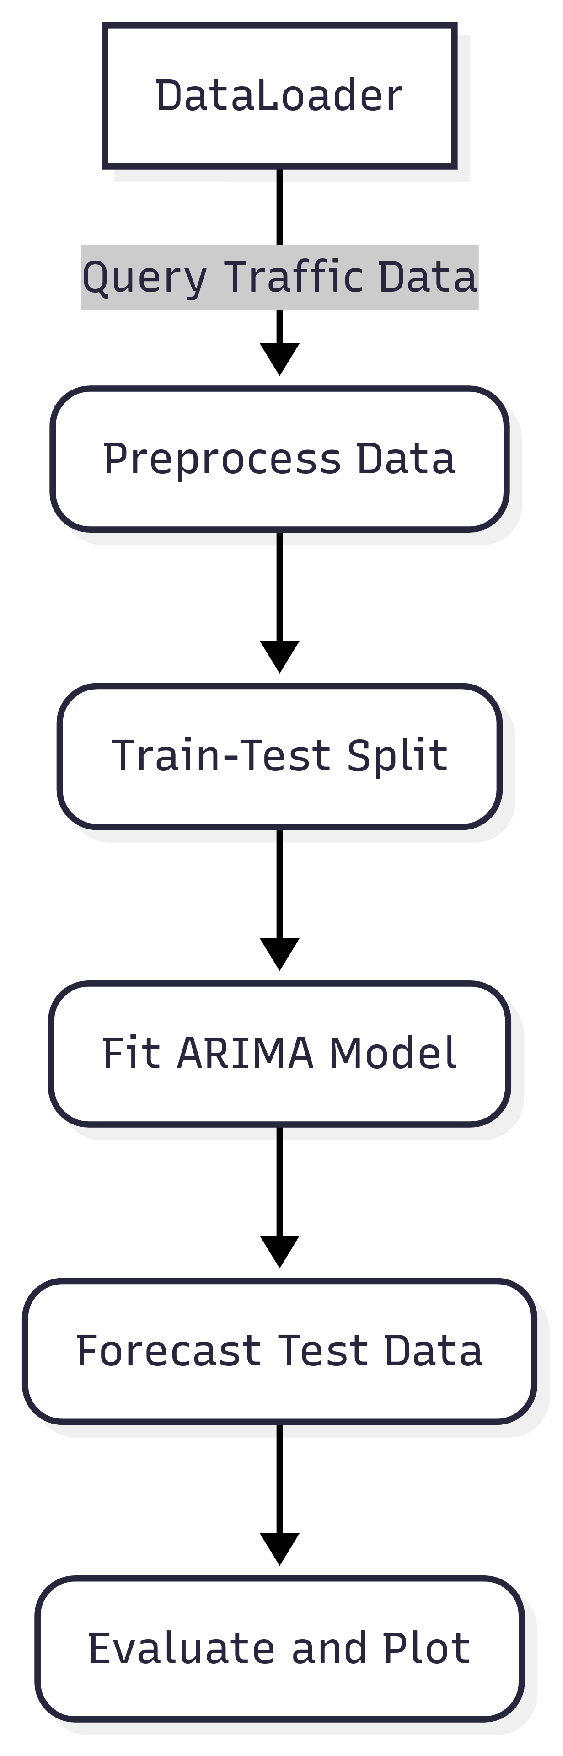
\includegraphics[width=0.2\textwidth]{images/design-implementation/arima.pdf}
  \caption{Architecture diagram of ARIMA predictive modelling}
  \label{fig:arima-arch}
\end{figure}

\subsubsection{Neural Network Model (LSTM)}
An architecture diagram for this model is provided in \fig{lstm-arch}. The design of this model is far more complex, as it is a neural network similar to that of the MLP in the next section. In this model, our DataLoader queries traffic and event data, which is passed to the FeatureEngineering module to add all the features and drop unused columns. We then perform some preprocessing by splitting the data into the same test-train split of 80-20\% and scaling the data. A peculiarity of this model is the need to create time-series windowed data from the generated data before using our Trainer class to train the model. Once this is done, we perform two forecasts before evaluating and plotting the results. We delve into more detail in the sections below. This model was abandoned, as discussed in the \textbf{\hyperref[link:lstm-results]{results}}, and therefore, no optimisations past the architecture below were performed.

\begin{figure}[!ht]
  \centering
  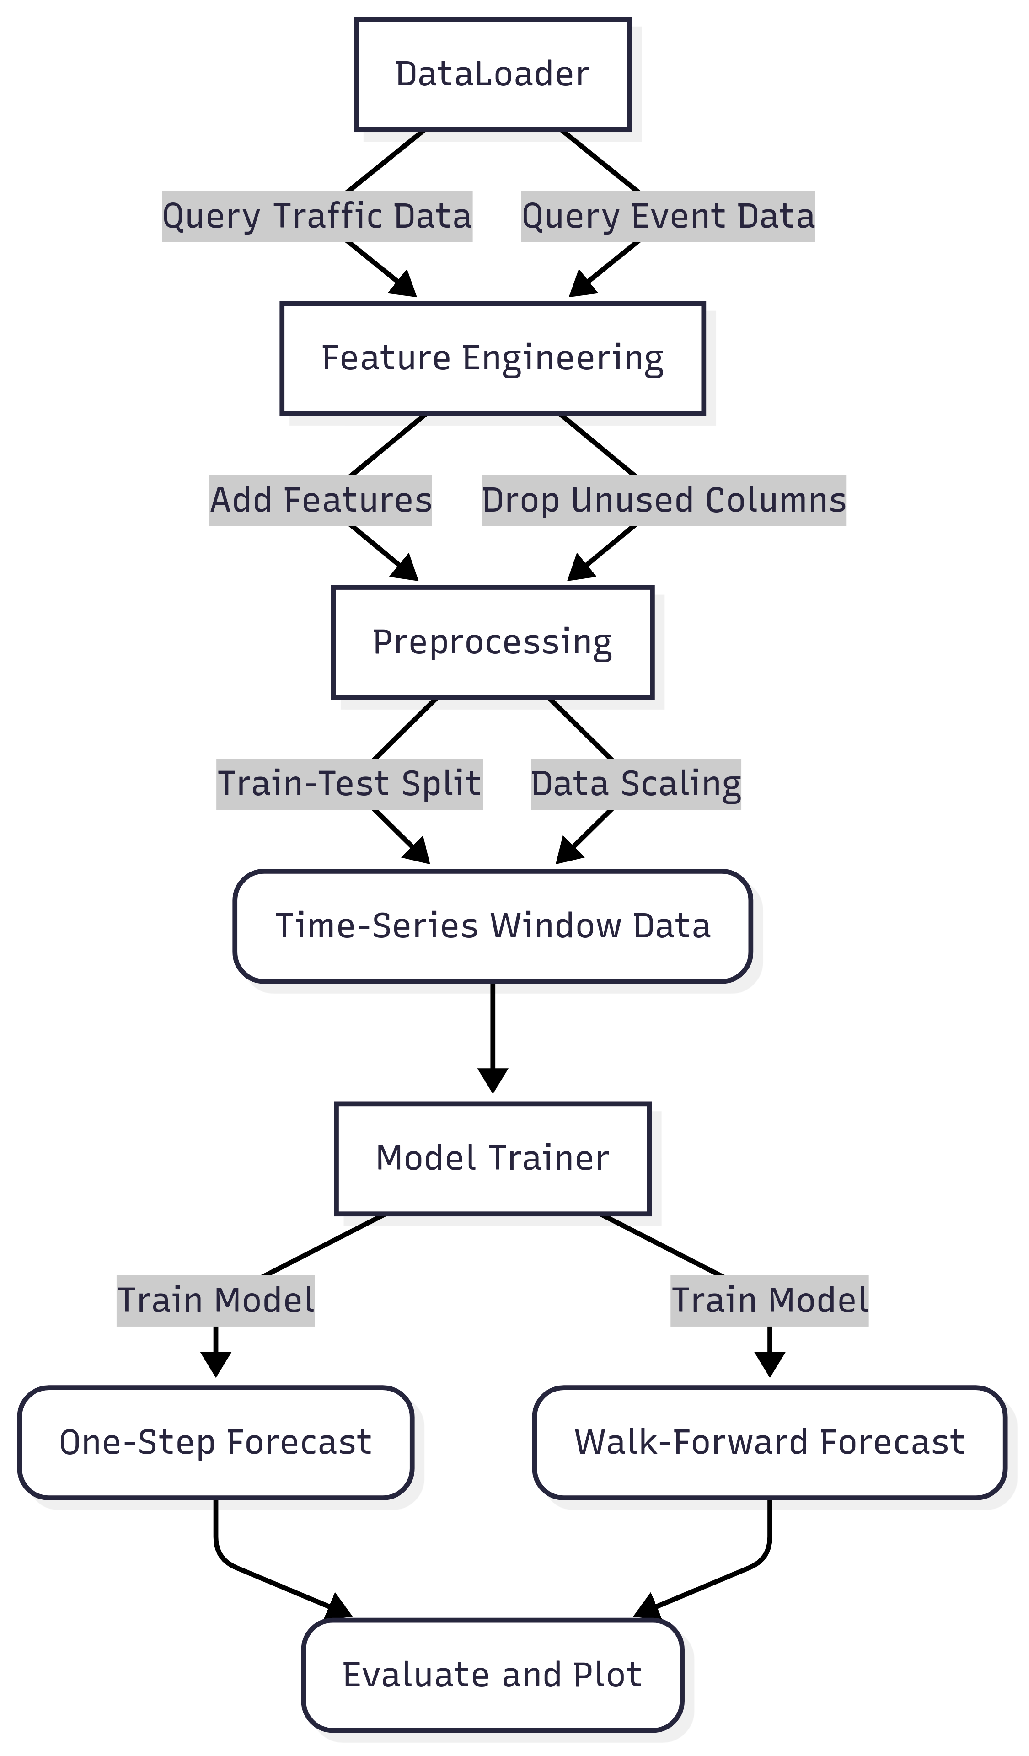
\includegraphics[width=0.5\textwidth]{images/design-implementation/lstm.pdf}
  \caption{Architecture diagram of LSTM predictive modelling}
  \label{fig:lstm-arch}
\end{figure}

\paragraph{Data Scaling}
\label{link:data-scaling}
We applied MinMax scaling for this model to ensure all input features fall within the same range. This is crucial because LSTMs are sensitive to the scale of data. Unscaled features can lead to unstable training and slower convergence; therefore, scaling helps the model learn temporal patterns more effectively, leading to higher precision \cite{sharma_study_2022}.

\paragraph{Time-Series Window Data}
Creating time-series windowed data is necessary for LSTM models as they are designed to learn from sequential patterns over time. The model can capture temporal dependencies and trends spanning multiple time steps by structuring the data into fixed-length input sequences (windows). This approach enables LSTMs to use historical context when forecasting future traffic speeds, which is essential for this task. We implemented this function using a variable window size that can be tweaked.

\paragraph{LSTM Architecture and Training}
For the architecture, we use a typical simple LSTM network with two layers of 100 units, each with a dropout of 10\%. This model is optimised using an ADAM optimiser \cite{kingma_adam_2017}, EarlyStopping to ensure no overfitting or wasted computational power over 50 epochs, and a validation split of 20\% of the previous 80\% training data. This ensures we train on a part of the data, optimise our model learning over another part, and then perform the final testing on another, completely separating them to ensure valid results.

\paragraph{Forecasts}
For this model, we implement two types of forecasts: a One-Step Forecast and a Walk-Forward Forecast. Since the LSTM model is most suitable for short-term forecasting, it should excel at a one-step forecast, which uses the model to predict a single step ahead. A walk-forward forecast, however, attempts to consecutively predict many steps in advance to construct a more long-term forecast, which we predict will be an issue for the LSTM.

\subsubsection{Neural Network Model (MLP)}
\label{link:mlp-design}
We provide an architecture diagram for this model in \fig{mlp-arch}. In this model, our DataLoader queries traffic and event data, which is passed to the FeatureEngineering module to add all the features and drop unused columns. We then perform some preprocessing by splitting the data into the same test-train split of 80-20\% % and scaling the data. Finally, we train the model using the Train class, and a forecast of the train data is performed, evaluated and plotted while also saving the trained model and scalers for future use in the next step of our project, the simulations. We delve into more detail in the sections below. We selected this model as the most promising, and therefore, we performed several optimisations.

\begin{figure}[!ht]
  \centering
  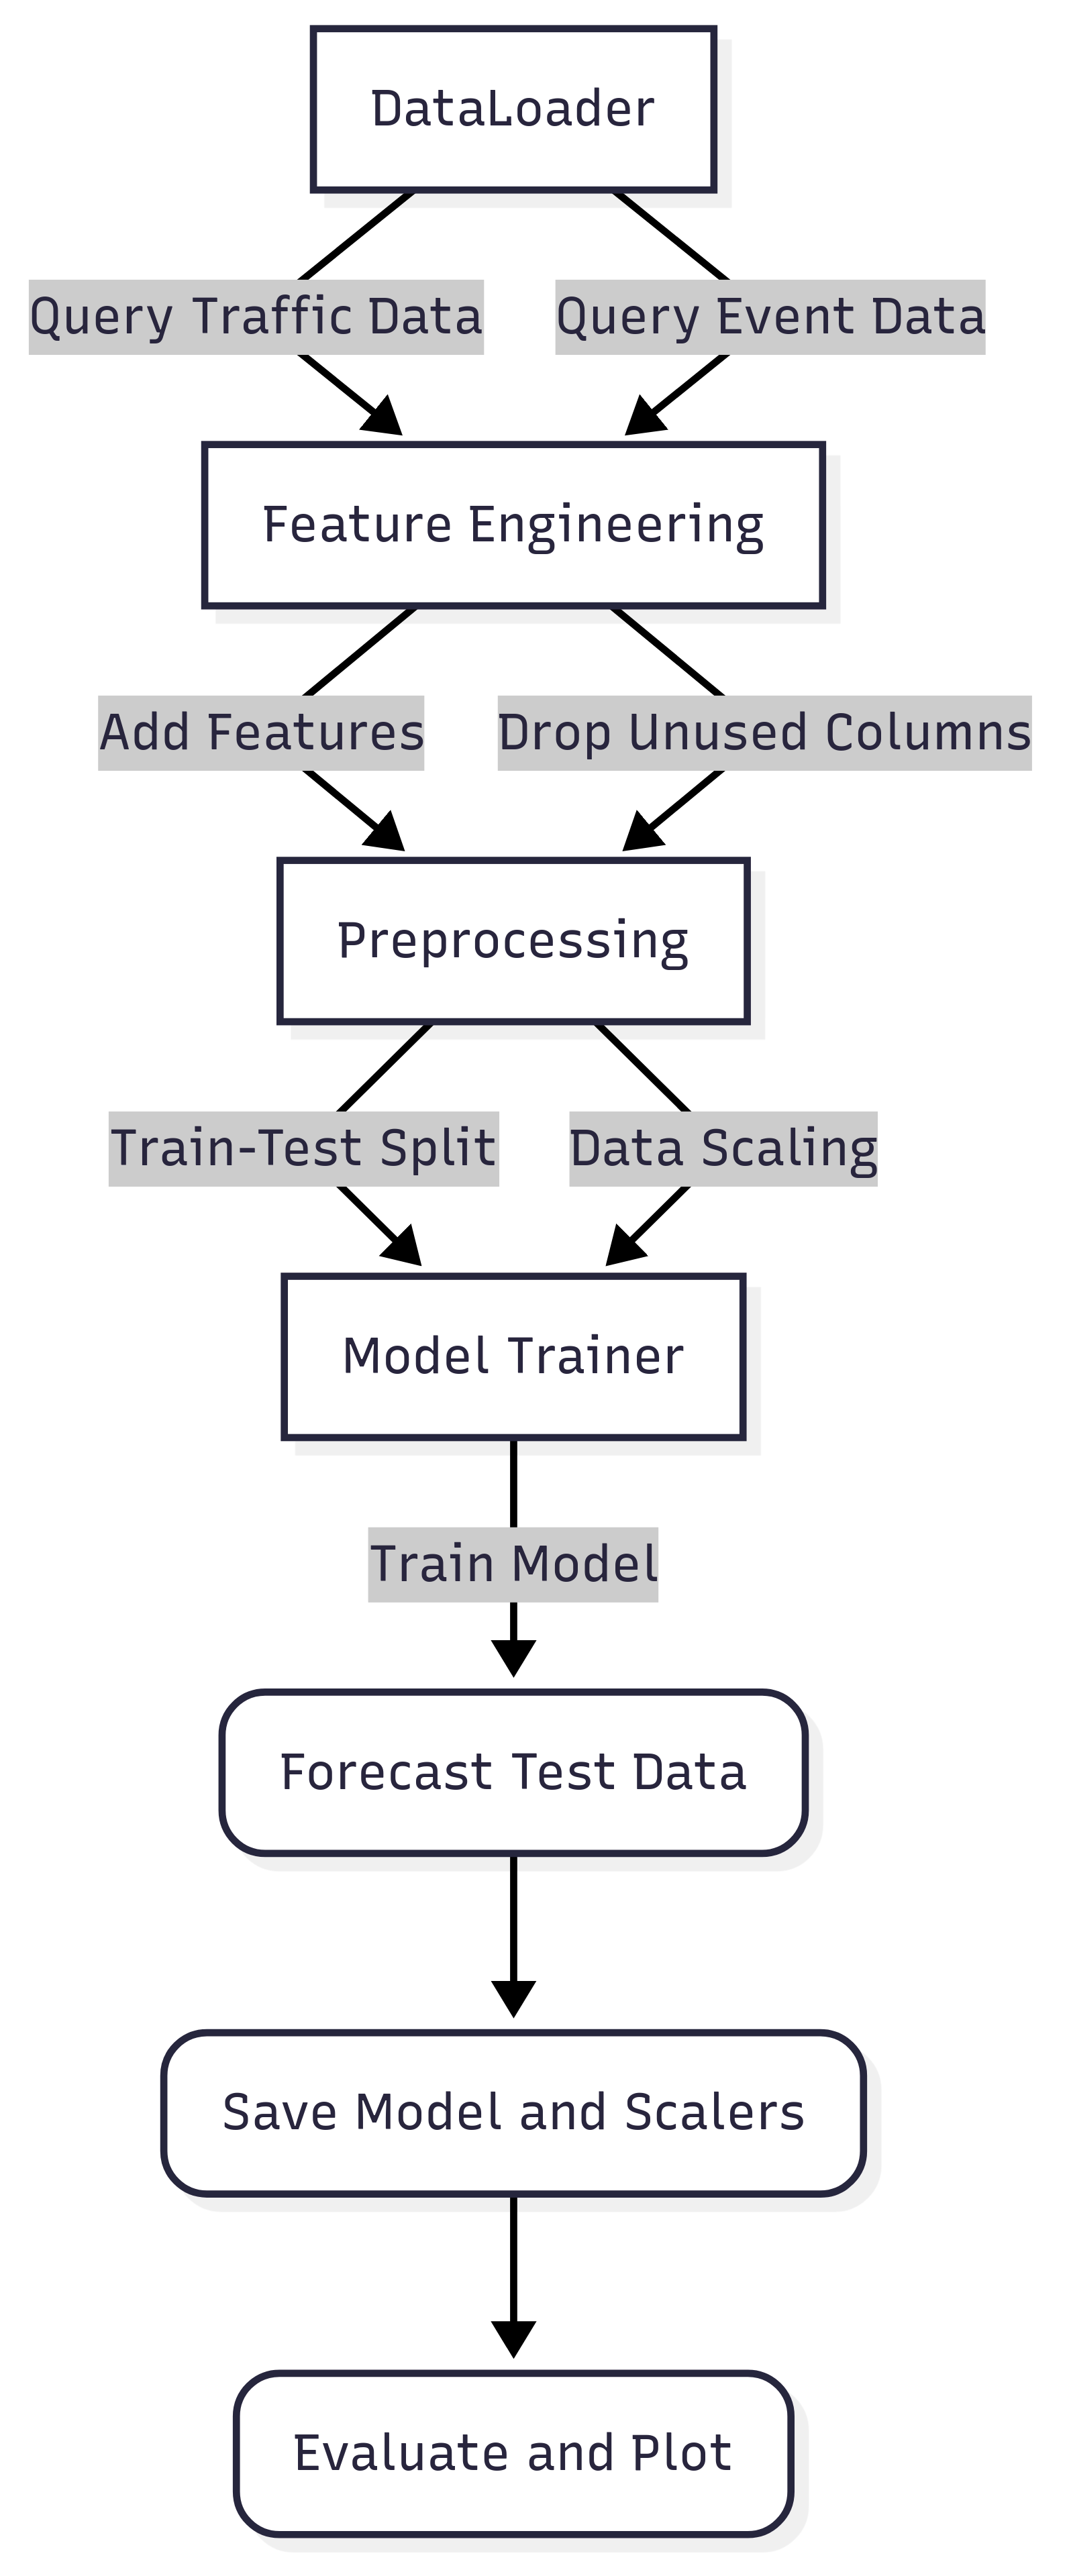
\includegraphics[width=0.38\textwidth]{images/design-implementation/mlp.png}
  \caption{Architecture diagram of MLP predictive modelling}
  \label{fig:mlp-arch}
\end{figure}

\paragraph{Data Scaling}
We applied robust scaling to this model to ensure all input features fall within the same range. This is for the same reasons as discussed in \textbf{\hyperref[link:data-scaling]{data scaling}}. However, here, we use robust scaling instead of MinMax since it is tolerant of outliers, ensuring our models perform better even with outliers that may be present in the traffic data by using the inter-quartile range instead of the minimum and maximum to scale \cite{noauthor_robustscaler_nodate}.

\paragraph{Modular MLP Architecture and Training}
\label{link:modular-mlp-arch}
For the MLP architecture, we make use of a modular architecture. Instead of specifying a certain number of layers, neurons per layer, dropout rate, among others, we specify a modular architecture with several options for each parameter. This allows us to then tune the parameters in \textbf{\hyperref[link:hyperparam-tuning]{hyperparameter tuning}}, achieving the best architecture within our search for the required task. The base architecture consists of a dense input layer, followed by several hidden layers and an output layer. As with the LSTM architecture, we use a validation split of 20\% of the previous 80\% split training data, ensuring the separation of the three stages. We discuss the hyperparameters and training of this architecture in more detail in \textbf{\hyperref[link:hyperparam-tuning]{hyperparameter tuning}}.

\paragraph{Outputs}
To enable the use of the trained models in the remainder of the project, the flow of training the MLP model saves the trained model weights and the scalers used to scale the data. This will allow us to load the model weights, use the same scalers on new data, and generate predictions in the next stage.

\subsubsection{Hyperparameter Tuning}
\label{link:hyperparam-tuning}
This section covers hyperparameter tuning and model training in more detail, specifically for the MLP model as our choice of model for predictions. To perform hyperparameter tuning, we set up a modular architecture, as described above, and then ran a random search over 100 trials to determine the optimal configuration of hyperparameters for the network. During this search, we focus on minimising the validation loss and achieving the highest validation accuracy while also implementing Early Stopping to prevent overfitting. We present the hyperparameters chosen for search in \tab{hyperparameters-mlp}.

\begin{table}[!ht]
    \centering
    \caption{Hyperparameter grid for search on MLP architecture}
    \label{table:hyperparameters-mlp}
    \resizebox{\textwidth}{!}{%
    \begin{tabular}{|l|l|l|p{8cm}|}
    \hline
    \textbf{Hyperparameter} & \textbf{Type} & \textbf{Choices / Range} & \textbf{Description} \\
    \hline
    \texttt{units\_input} & Integer & \{64, 128, 256\} & Number of neurons in first dense (input) layer. \\
    \texttt{activation} & Categorical & \{relu, tanh\} & Activation function used in each dense layer. \\
    \texttt{dropout\_input} & Float & [0.1, 0.3], step=0.1 & Dropout rate applied after the input layer. \\
    \texttt{num\_layers} & Integer & [2, 4] & Total number of hidden layers. \\
    \texttt{units\_i} (per layer) & Categorical & \{64, 128, 256\} & Number of neurons in each hidden layer. \\
    \texttt{dropout\_i} (per layer) & Float & [0.1, 0.3], step=0.1 & Dropout rate applied after each hidden layer. \\
    \texttt{optimizer} & Categorical & \{adam, rmsprop\} & Optimization algorithm used for training. \\
    \hline
    \end{tabular}
    }
\end{table}

The choices or ranges shown above were chosen to balance a range of testing with computational efficiency. In summary, we chose three values for each hyperparameter, except for the categorical ones, where we chose only two. For all the choices, we used the standard range typically used in ML, specifically MLP structures. As it would be unfeasible to run this hyperparameter search for each model of sensor or one single sensor over the whole training period, we will run the search on one specific sensor and direction as in the \textbf{\hyperref[link:data-analysis]{data analysis}}. We will then extrapolate the findings for all other sensors and the whole training cycle.

\subsubsection{Evaluation Strategy}
We now present a more detailed description of the model’s evaluation strategy, including the metrics we focus on and the plots and forecast visualisations.

\paragraph{Loss Function Metric}
Several metrics can be used to evaluate the model’s performance and use it in the loss function during training. As traffic speed is a continuous variable, this problem is a regression task, for which the most common metrics include MAE and MSE. We decided to use MSE as it performs better with the highs and lows that are common in traffic speed prediction. 

\paragraph{Forecast Visualisations}
Forecast prediction visualisations are an excellent tool for understanding how the model functions, comparing changes made, and assessing the model’s accuracy. These visualisations are also the ones used in the \textbf{\hyperref[sec:results-discussions]{results section}}. The designed plots overlay the actual traffic speeds with the model’s forecasted ones on the test dataset. Since this spans over a few months, each Plot generated was designed to show the whole timeline, the middle 10\%, and the middle 3\%. These zoomed-in versions allow the researcher or reader to understand the model over months, weeks, or days and gather a finer understanding of trends on different scales.

\paragraph{Metrics Gathering}
Finally, we discuss the gathering of metrics from the models. For this task, our training class evaluates the trained model against the test data, using MAE, MSE, RMSE, and MAPE accuracy. From the options for loss metrics, we add RMSE as the squared value of MSE to standardise units and MAPE, as it allows us to compare our results with other datasets and studies. These four metrics are the most common in most works in the area. These metrics are then saved to a CSV file, along with the metadata of that model (dates trained on, platform ID, sensor ID).

\subsection{Traffic Simulation}
We developed a semi-automated pipeline to streamline our simulation process using SUMO, enabling efficient evaluation and comparison of congestion management strategies. This pipeline integrates several key components, including automated map generation, predictive model training, demand simulation, and congestion strategy implementations. With this pipeline, we can simulate various scenarios reflecting real-world conditions and rigorously assess the impact of different congestion management techniques on overall traffic efficiency and metrics.

\subsubsection{Design Decisions}
\label{link:sim-design-decisions}
\paragraph{Congestion Management Strategy}
Firstly, we consider the choice of a congestion management strategy to simulate. As covered in the \textbf{\hyperref[link:cmt]{background chapter}}, many congestion management strategies can be applied. The most common ones are VSL, Dynamic Rerouting, or Ramp Metering. As ramp metering is used in motorways, and we focus on venues that do not have motorways as their main access point, we discard this option. The choice between VSL and Dynamic Rerouting is more fine-grained. However, we chose VSL as our strategy for the following reasons:
\begin{itemize}
    \item Most venues explored have one single point of entry. Using dynamic rerouting as a congestion management approach would not reveal results, as any alternative route would increase travel time by more than the traffic through the initial route.
    \item SUMO simulations already perform dynamic rerouting internally. While disabling this is possible, we prefer to focus on a congestion management strategy that proves results compared to a typical baseline.
    \item Implementing a VSL strategy using SUMO and TraCi is powerful and allows for fine-grained control and comparison.
\end{itemize}

\paragraph{Simulation Area}
We now discuss choosing an area of the city to run the simulation. There were several considerations towards this choice, namely:
\begin{itemize}
    \item An area large enough to measure the whole network effect, not only just local road segments, but small enough that it would be computationally feasible to simulate.
    \item An area that contains event venues to measure the impact of events on the congestion.
    \item An area for which we have enough traffic sensor data to generate demand.
\end{itemize}

The best area that fit all these requirements was the area containing both the Etihad Stadium and Co-Op Live venues, for which we had two separate sensor platforms covering an area of about 1.27 miles. The area's boundary is detailed in \fig{sim-area}, with labels for both the venues and the sensor locations.

\begin{figure}[!ht]
  \centering
  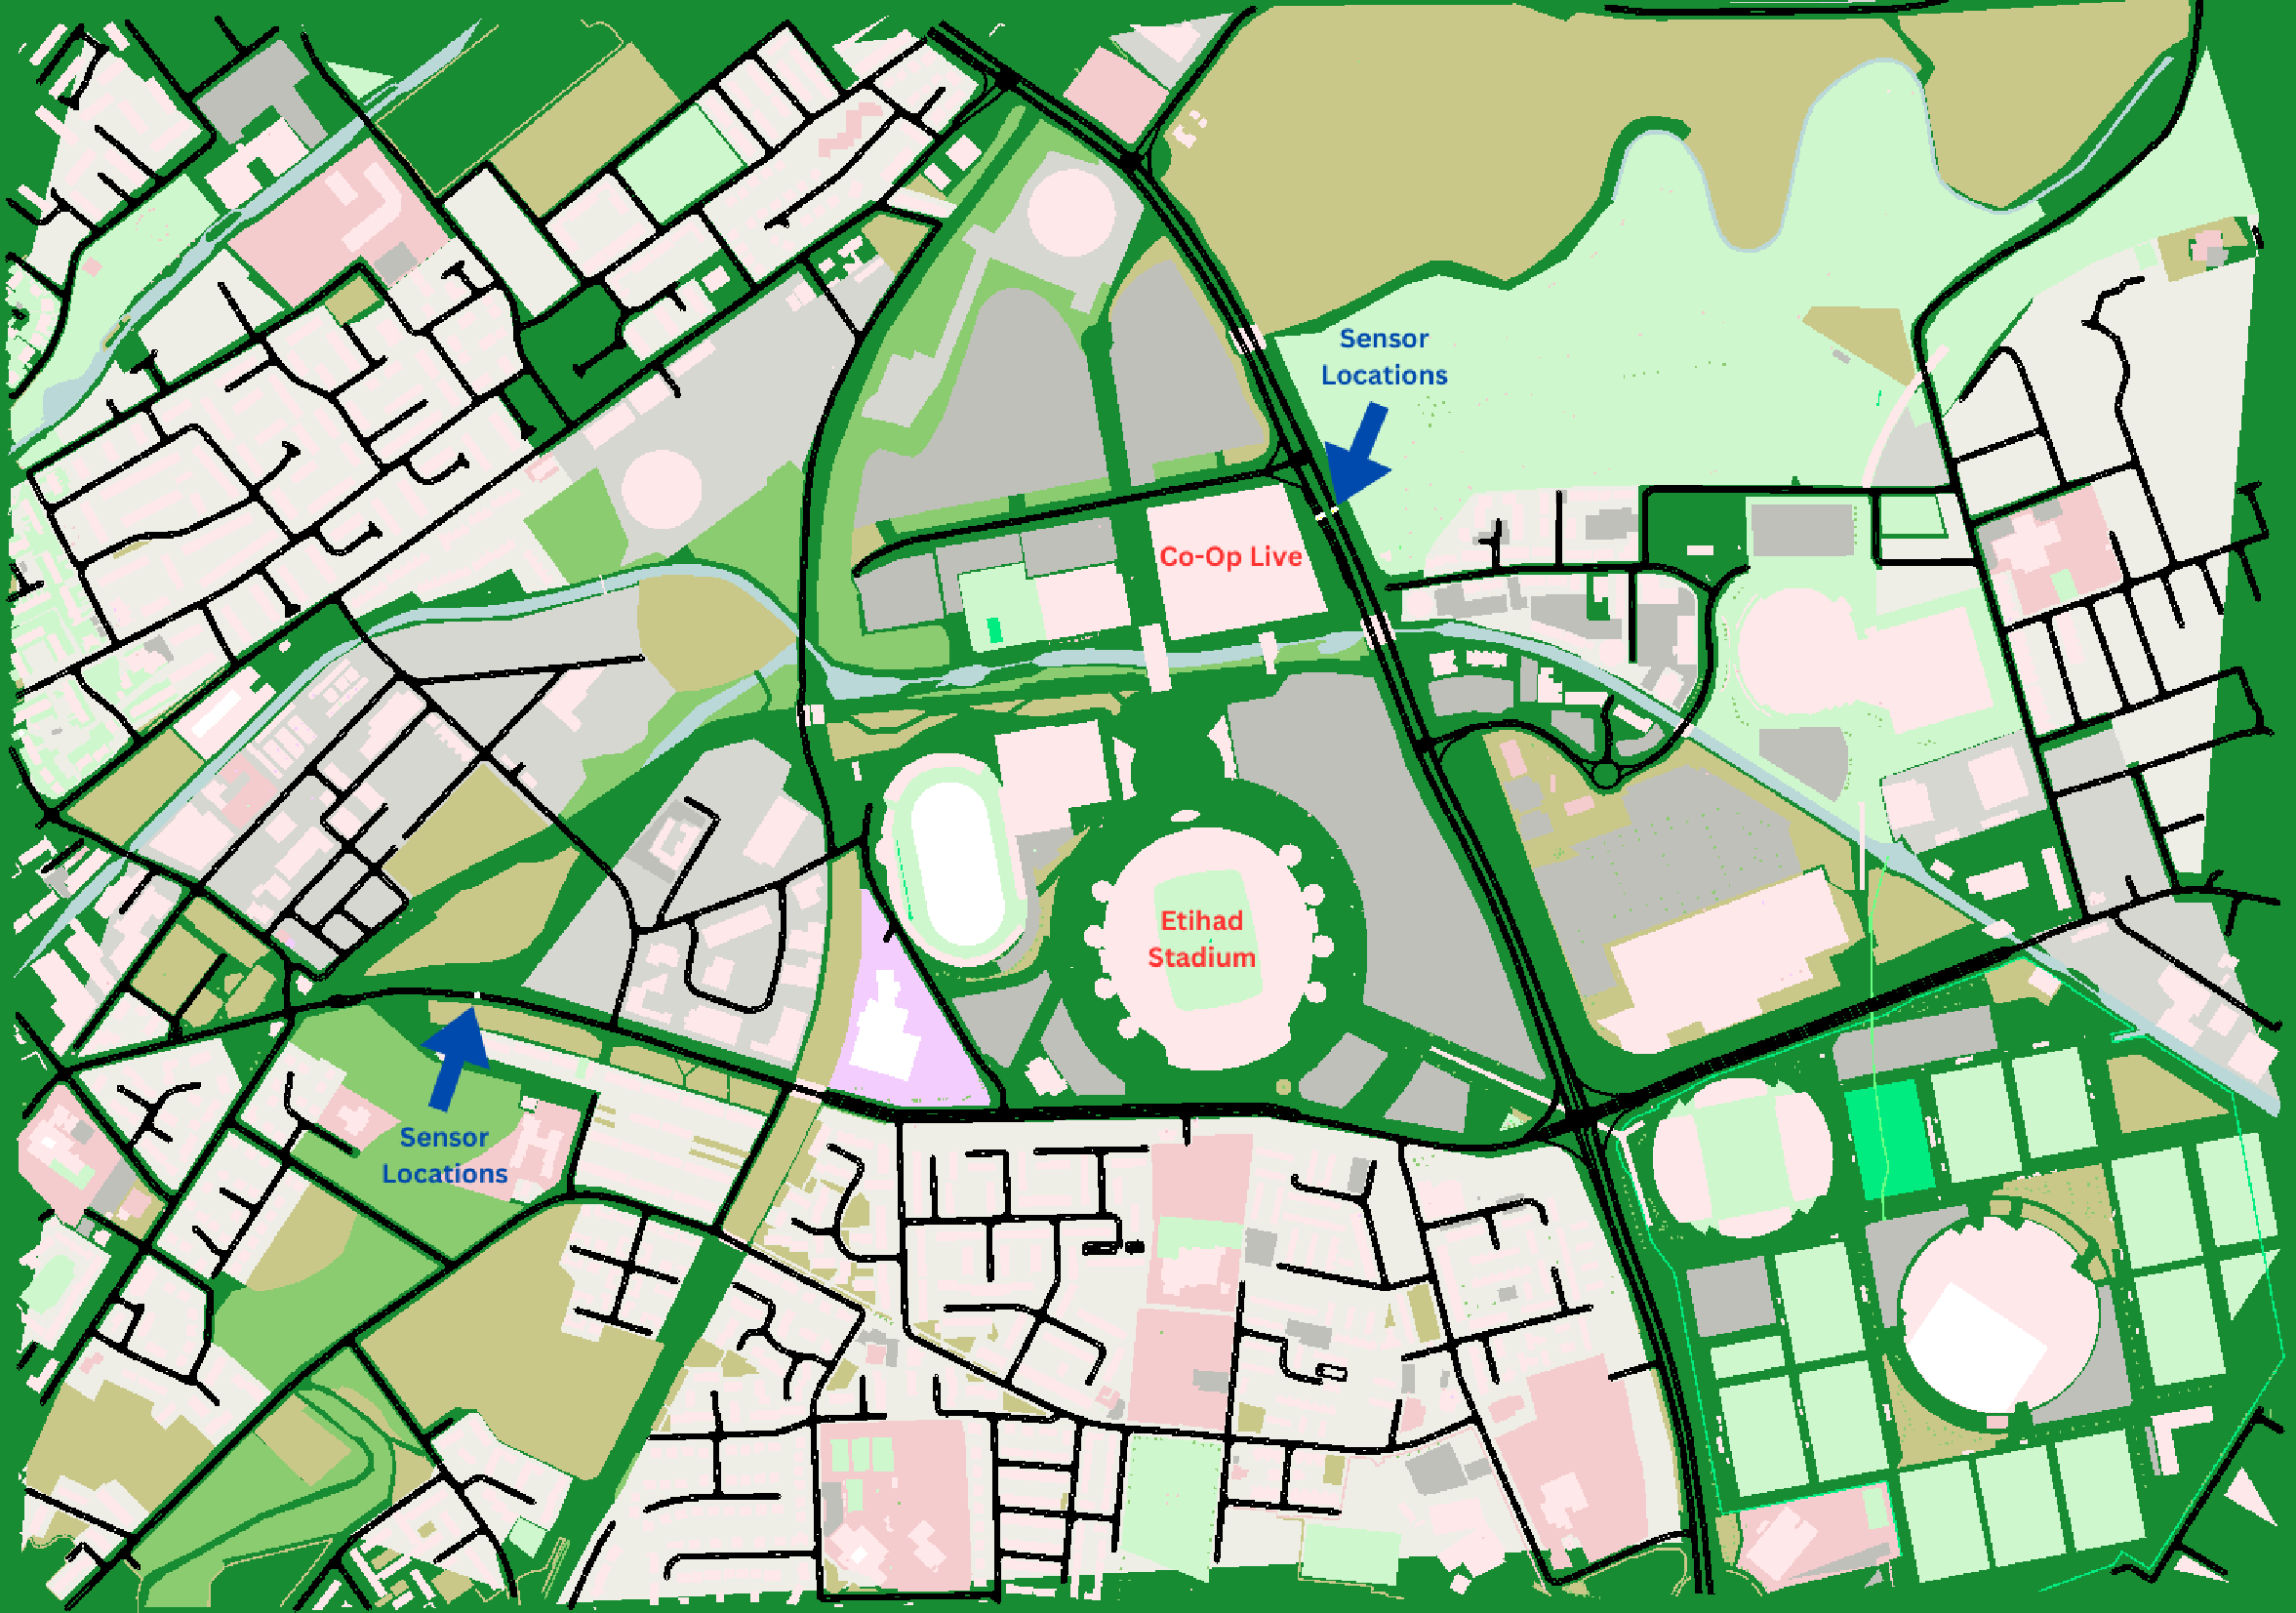
\includegraphics[width=\textwidth]{images/design-implementation/sim-area.pdf}
  \caption{Area boundary for simulation with labels}
  \label{fig:sim-area}
\end{figure}

\paragraph{Simulation Timeline}
Another design decision is related to the timeline of the simulation that we will run. It is computationally infeasible to run simulations for all the days of data that we have collected. Our main requirements are to run simulations over general and event days. We will run simulations on the following days to ensure a statistically significant sample.
\begin{itemize}
    \item 2024 Simulations: This batch of simulations covers 16 distributed days over 2024, specifically, the 1st and 15th day of each month from March to October.
    \item Event-Day Simulations: This batch of simulations covers 9 distributed days over 2024, manually chosen to be uniform around the year and to contain only days where an event occurs in either venue within our boundary.
\end{itemize}

\paragraph{Performance Metrics}
Finally, we discuss the possible performance metrics used to evaluate the strategies during simulation, the ones chosen and the reasons behind them. Many possible evaluation metrics exist in traffic management, and SUMO makes many of these easily accessible. Options include travel time, route length, waiting time, time lost, time spent on a specific edge (road segment), such as the edge closest to a venue, the number of vehicles, CO2 emissions, and others. To fully evaluate our strategies, we will focus on overall average network metrics instead of local ones. This means focusing on metrics that measure congestion or effect over the whole network map instead of focusing on just edges close to venues that may represent a significant improvement locally but then lead to congestion elsewhere in the network, allowing for real-world representative results.

After analysing all these metrics, we decided to focus on three that are the most descriptive: CO\sub{2} emissions, trip duration, and time loss. Trip duration and time loss metrics help ensure that any congestion management techniques applied either reduce or maintain how long an average trip takes or the time lost in traffic during these. CO\sub{2} emissions are one of the focuses of this project, where a reduction in CO\sub{2} emissions signifies a successful congestion management technique, reducing congestion and stop-and-go traffic \cite{hofer_large_2018}, but also shows the impact the technique can have on the environment.

\subsubsection{Map Generation}
This section details the map generation of the simulation. As we have selected an area to simulate, we now require converting this area into a simulation in SUMO. This includes the general map area and all the roads, junctions, and traffic lights.

\paragraph{osmWebWizard} osmWebWizard is a tool supplied with SUMO that assists in this task. It generates a SUMO simulation based on a selected area and generates random traffic for the simulation. Even though this latter feature will not be helpful to use as we will be generating our own traffic, the tool can convert a general area into a realistic simulation of that environment.

\paragraph{Assumptions}
When generating a simulation map using this tool, there are a few assumptions taken that we detail below:
\begin{itemize}
    \item As we are only interested in car traffic, we add only lanes usable by car traffic.
    \item All traffic lights in the simulation run with a fixed length cycle set by osmWebWizard in “adaptive” mode, which adapts the cycles according to traffic. While the adaptive mode should be representative, the fixed cycle time used in the real world is unknown.
\end{itemize}

\subsubsection{Prediction Generation}
Our simulations will require the use of predictive speed values for the predictive congestion management techniques. We discussed the training of models in detail in the \textbf{\hyperref[link:mlp-design]{MLP design}}. In this section, we will explore the training of these models in batches and the generation of predictions from these that will feed into our simulations.

\paragraph{Batch Training}
Taking advantage of our modular approach to the predictive model implementation, we developed a small tool, \verb|batch_training.py| in the \verb|model| directory in the repository (\hyperref[appdx:a]{Appendix A}), that trains models for all the sensors available. As discussed previously, some of these sensors had significant malfunctions that made them unfeasible for our purposes. To prevent this, the tool trains only models that, during the specified period of data, contained over 80\% of data points. Running this tool will train all the possible models, exporting data required for analysis of predictive accuracy, but also to be used in the next step, prediction generation.

\paragraph{Prediction Generation}
To generate the predictions required for simulation, we developed another tool, \verb|predict.py| in the \verb|model| directory in the repository (\hyperref[appdx:a]{Appendix A}), that generates predictions in batch for specified sensors and date ranges. In our case, this tool will be used to generate the predictions for the sensors within the simulation boundaries and for the dates outlined in the \textbf{\hyperref[link:sim-design-decisions]{design decisions}}. This tool saves the predictions to CSV files that are ingested during the simulation and creates simple plots to visualise any errors in predictions easily.

\subsubsection{Demand Simulation}
The simulation pipeline's next step is generating demand according to real-world data. This will allow us to test our techniques in similar environments to the real world, which is especially important with predictive algorithms. The conditions in the simulation need to be as similar as possible for the predictive algorithms to function correctly. To achieve this, we cover two main aspects: the automated placement of the real-world traffic sensors into the simulation and the actual demand generation based on those sensor readings.

\paragraph{Virtual Sensor Placement}
An architecture diagram for this task is provided in \fig{sensor-placement}. There are many types of sensors in SUMO. However, induction loop sensors are the best conversion for our data, providing both speed and count aspects, and therefore, we will place them as such. Since the traffic data we have is for all lanes across an edge, but each lane in SUMO requires a separate sensor, any data converted to or from simulation is divided or summed across the number of lanes, accordingly.

\begin{figure}[!ht]
  \centering
  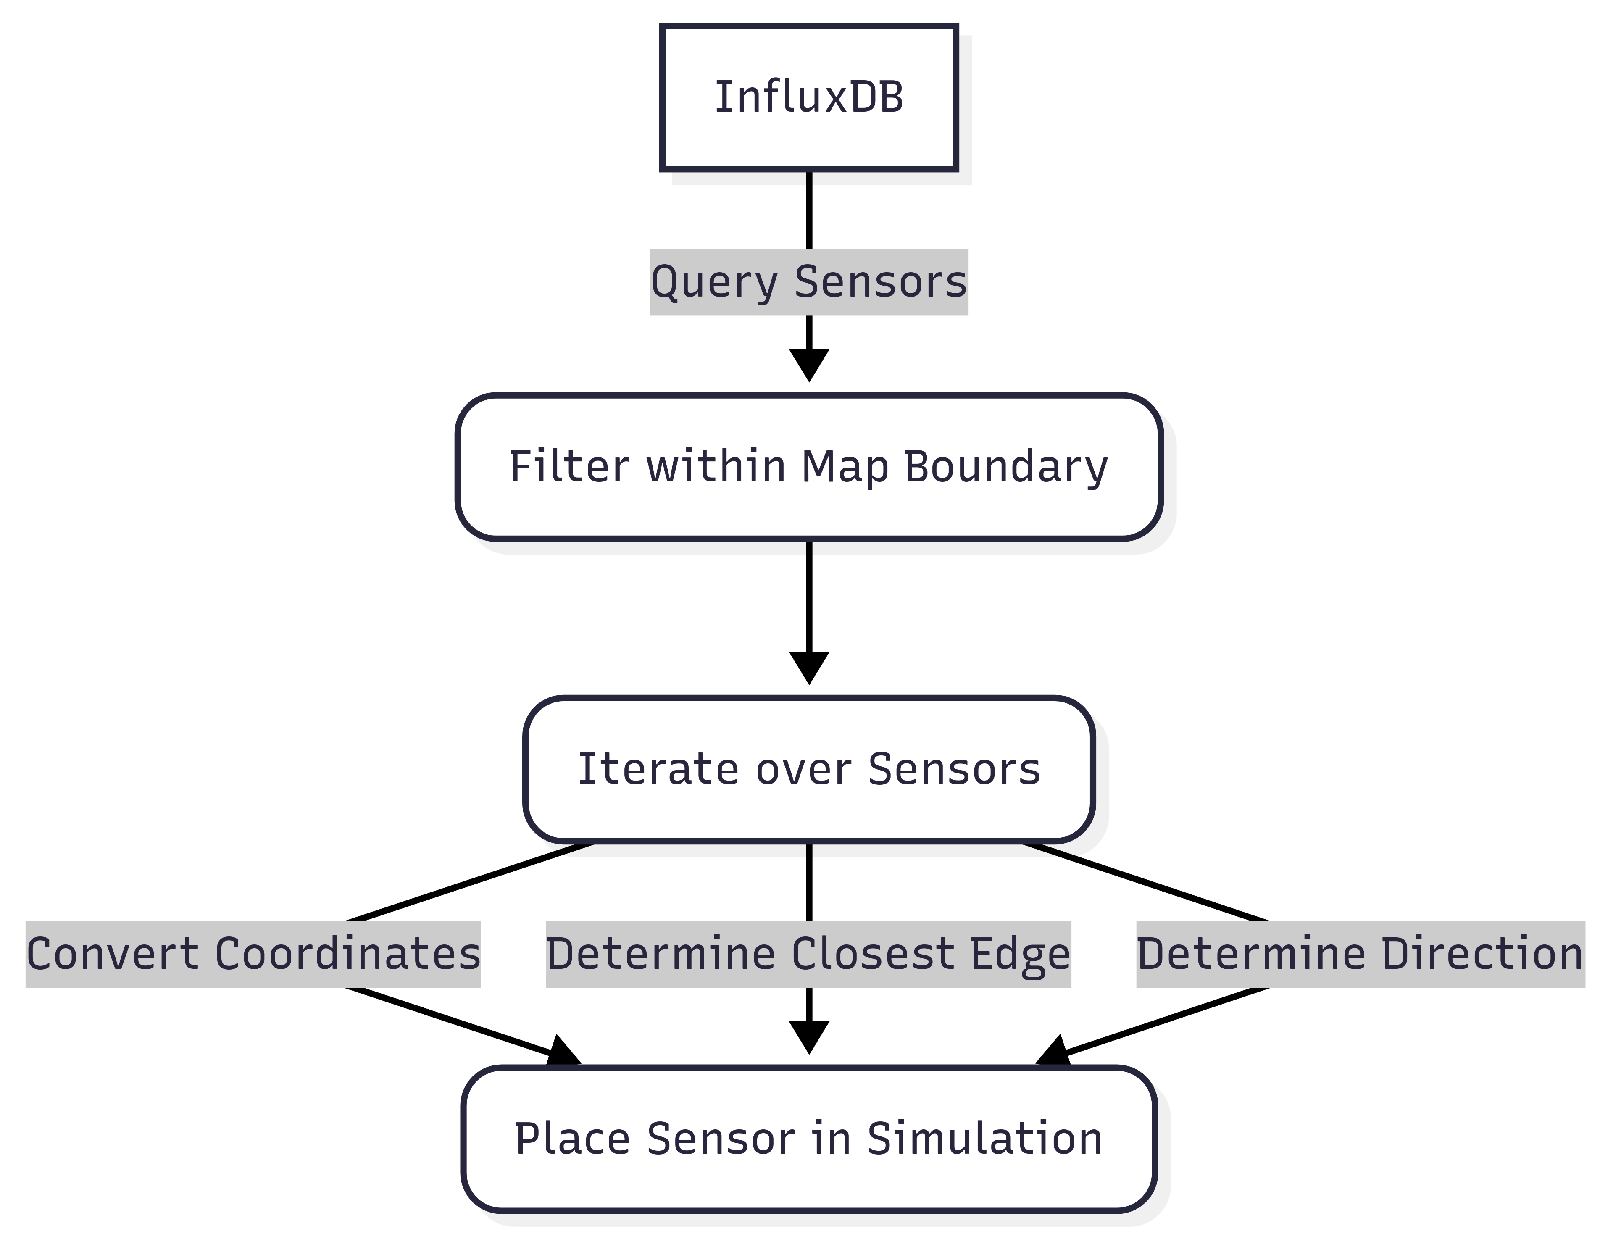
\includegraphics[width=0.5\textwidth]{images/design-implementation/sensor-placement.pdf}
  \caption{Architecture diagram of automated simulation sensor placement}
  \label{fig:sensor-placement}
\end{figure}

We have developed a tool for sensor placement that works by querying InfluxDB for all sensors and reducing them down to sensors within the boundary of the specific simulation. We then place these by converting their real-world coordinates to coordinates within the simulation map, and then we use a point-to-polyline algorithm to determine the road edge closest to these. Once this is found, we place the sensor according to its direction metadata by comparing the lane directions of that edge. The tool completes by creating an additional file for the simulation that adds this information so that SUMO can add these sensors during runtime.

\paragraph{Demand Generation}
An architecture diagram for this task is provided in \fig{demand-conversion}. The next step in our simulation pipeline is to generate the required demand in the traffic network that illustrates the real-world conditions during each day of the simulations. To do so, we once again built a small tool that used our data sources and SUMO-provided tools to generate demand files for use in the SUMO simulation that relayed the real-world demand during that day. One issue with this method is that demand can only be generated using traffic counts, not speeds. While the tool includes the speed data in the intermediate edge data files, the \verb|routeSampler| tool only uses the counts.

This tool works by querying speed and count data for the specified simulation day, and also generates random trips for the simulated cars. Once this is done, we load the sensor placements and SUMO network that we will base our calculations on, and apply scaling to prevent total network congestion. With this data, we generate edge data files. These intermediate files contain the required speeds and counts of the edges for which we have sensor data. The challenges related to the use of counts, random trips, and scaling are detailed in the \textbf{\hyperref[link:trip-info]{challenges section}}.

With this data, the SUMO routeSampler tool \cite{noauthor_turns_nodate} generates the demand files for the network, creating as much demand as needed to achieve the required vehicle counts for the edges where we have count data. This tool uses heuristic sampling to generate demand that achieves the required constraints of the counts we generated earlier. Since our data sources are limited, this sampling introduces randomness on edges that are further away from our sensor locations, as we have no available data from which to sample.

\begin{figure}[!ht]
  \centering
  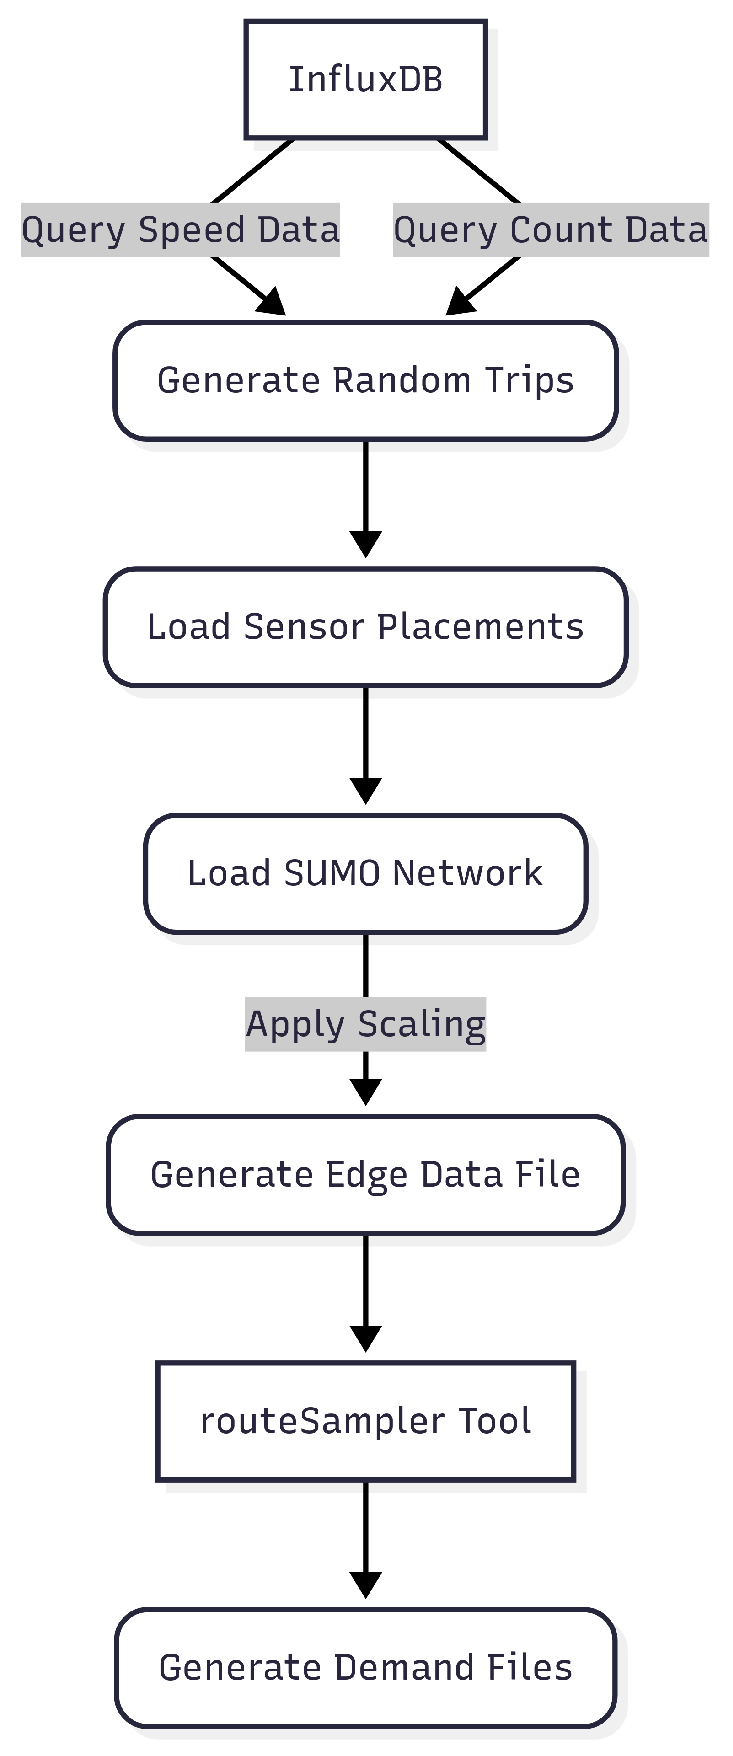
\includegraphics[width=0.3\textwidth]{images/design-implementation/generate-demand.pdf}
  \caption{Architecture diagram of automated simulation demand generation}
  \label{fig:demand-conversion}
\end{figure}

\subsubsection{Congestion Management Strategies}
As discussed previously, we will compare different congestion management strategies in simulation using a VSL approach. The strategies will each use different algorithms to alter the maximum speed limit on the road edges for which we have traffic data. We will use the data from the simulation to compare these. We will compare baseline, reactive, and proactive strategies, which are detailed below.

\paragraph{Baseline Implementation}
We will simulate our baseline using no congestion management technique. This means the speed limit for the edges will remain at its maximum during the whole simulation. As another control technique, we implement a second baseline (Lower Limit) that uses a lower speed limit for all these edges. This is to ensure that any results retrieved are indeed from a valid congestion management technique and not from a lower fixed speed limit alone. This lower speed limit is set to the same value as the reactive technique's lowest used, described in the next section.

\paragraph{Reactive Implementation}
A few reactive strategies can be used for the reactive implementation. These include using a moving average or a rule-based version. The moving average attempts to take advantage of a rolling average of traffic speed and apply this value to maintain constant speeds. The rule-based version uses a fixed set of rules defined in advance and usually tuned to the particular edge it is used on to derive the speed limits to set. This rule-based technique is the most used in current deployments, and initial testing with the moving average technique yielded inconsistent results with our simulation setup. Therefore, our implementation makes use of a rule-based technique described below.

Our rule-based implementation works using the current speed and density of vehicles on an edge and some hyperparameters that can be tuned. The rules are shown in \fig{reactive-code}. To summarise, we reduce speed heavily if the traffic density is over a high-traffic threshold. If not, but the current speed is under a less dramatic speed limit, we set it to that. We use the default maximum speed limit if neither of the other conditions applies. This type of rule-based system is typical for use in reactive VSL systems, for which we have adapted its use here \cite{grumert_characteristics_2018, allaby_variable_2007}.

\begin{figure}[!ht]
  \centering
   \begin{minted}{python}
    cur_meas = traci.edge.getLastStepMeanSpeed(edge)
    traffic_density = traci.edge.getLastStepVehicleNumber(edge)
    
    if traffic_density > HIGH_TRAFFIC_THRESHOLD:
        vsl = SPEED_REDUCTION_2  # Heavy congestion
    elif cur_meas < SPEED_REDUCTION_1:
        vsl = SPEED_REDUCTION_1  # Moderate congestion
    else:
        vsl = DEFAULT_SPEED_LIMIT  # Normal conditions
    \end{minted}
  \caption{Rule-based reactive implementation rules}
  \label{fig:reactive-code}
\end{figure}

To set the hyperparameters in this approach, we will run half of the “2024 Simulations” we described to set them according to the best results. To optimise computational efficiency, we will also add a timeout for the simulations, where if a simulation step takes more than 2 seconds, we discard that combination. This can be safely done, as a step taking this long means the whole network is congested and is, therefore, not a good combination.

\paragraph{Proactive Implementation}
For the proactive implementation, we use the predictions from our models in a few different ways to test the effectiveness of the proposed algorithm. The first and pure implementation is to set the speed limit to the output of the predictive model at that time step (in our case, 5 minutes, as this is the data frequency). This algorithm has a few inherent issues and optimisations that can be applied, especially concerning applicability to real-world use:
\begin{itemize}
    \item Since we are using a predictive model, it may make sense to use the predictions some time ahead instead of what the predictions at the current time step would be, attempting to anticipate traffic congestion further in advance.
    \item In a real-world scenario, it would be impractical to set the speed limit to a continuous number, such as 27.95 MPH, which is the pure output of our models. Instead, rounding would be necessary for drivers to be able to follow the limits. We need to investigate whether this rounding may impact the effectiveness of a prediction technique.
\end{itemize}

To enable the comparison of the strategies, our implementation consists of a pure predictive approach, as well as alterations to use prediction 30 minutes in advance and rounding to the nearest 2 or 5 MPH.

\subsubsection{Challenges Encountered}
The design and implementation of the simulations were, by far, the most challenging part of this project. Many challenges were faced, many of which we could overcome, while some still affected our results and may need further work.

\paragraph{Count-Generated Demand}
\label{link:count-demand}
The first and largest challenge was the limited demand generated through traffic count. The focus on speed was justified earlier due to its larger descriptive power. Since we can only generate simulation demand through count, we lose this descriptiveness, which may lead to inferior simulation outcomes. We will discuss the effects of this in the \textbf{\hyperref[link:demand-results]{results section}}.

\paragraph{Simulation Inefficiencies}
\label{link:sim-inef}
The second challenge concerns simulation inefficiencies and their separation from real-world traffic networks. Several inefficiencies are inherent in this type of simulation model, leading to inefficiencies in the network that cause overscaled congestion when modelling the same counts as real-world traffic. This can be from traffic light programming differences, sensor errors, or even map errors where junctions are improperly configured. Due to this, simulating with real traffic counts leads to completely congested networks and, therefore, unreliable results. To address this, we will scale down the traffic counts by 30\% before generating demand to ensure networks with realistic demand curves.

\paragraph{Random Trip Information}
\label{link:trip-info}
During demand generation, we require a list of “trips”, which are routes that the cars generated will follow. This can be made randomly or according to an Origin-Destination matrix, typically provided by a traffic authority, that contains the origins and destinations of trips in a traffic network. Unfortunately, TfGM does not provide these matrices, so we had to use random trips. This becomes another inefficiency, which can reduce the accuracy of the results.

\end{document}